\documentclass[9pt]{beamer}
\usepackage[utf8]{inputenc}
\usepackage[spanish]{babel}
\usepackage{newcent}

\usetheme{Warsaw}

\author{Gabriel Sanhueza}

\title[JHawanet Framework]{Software para la optimización de redes de distribución de agua potable}
\subtitle{JHawanet Framework}
%\setbeamercovered{transparent} 
%\setbeamertemplate{navigation symbols}{} 
\titlegraphic{
\includegraphics[height=1.5cm]{utalca1.eps}}
 
\institute [Universidad de Talca]{Defensa de Título\\ Universidad de Talca} 

\date{Agosto, 2020}



\begin{document}

    \frame{\titlepage}

    \section{Introducción}

    \subsection{Contexto}
    \begin{frame}
        \frametitle{Contexto}
        \begin{itemize}
            \item Escasez de agua
            \item Sistemas que deben estar las 24 horas del día activo
            \item Múltiples criterios para optimizar los sistemas de distribución
            \item Las redes de agua (RDA) involucran dos tipos de problemas:
            \begin{itemize}
                \item Problema de diseño
                \item Problema de operación
            \end{itemize}
        \end{itemize}
    \end{frame}

    \subsection{Problema}
    \begin{frame}
        \frametitle{Problema}
        
        \begin{columns}
            \column{0.6\textwidth}
            \begin{itemize}
                \item No se cuenta con las suficientes herramientas y tiempo para la correcta gestión de las redes de distribución de agua potable.
                \item El escoger las especificaciones es una tarea difícil debido a que hay que evaluar el rendimiento general del sistema.
            \end{itemize}

            \column{0.4\textwidth}
            \begin{figure}
                
\includegraphics[width=\textwidth]{assets/MunecosBlancos/Aproblemado.jpg}
            \end{figure}
        \end{columns}
    \end{frame}

    \subsection{Propuesta de solución}
    \begin{frame}
        \frametitle{Propuesta de solución}
        Aplicación de escritorio extensible que permita optimizar procesos de diseño y operación en RDA.

        Problemas implementados:
        \begin{itemize}
            \item Problema de diseño de RDA basado en el costo de tuberías.
            \item Problema de operación basado en el Régimen de bombeo.
        \end{itemize}
    \end{frame}

    \subsection{Objetivos}
    \begin{frame}
        \frametitle{Objetivos}
        
        \begin{itemize}
            \item Objetivo general    
            \begin{itemize}
                \item Diseñar y desarrollar una aplicación extensible de escritorio para optimizar el diseño y operación de una red de distribución de agua.
            \end{itemize}

            \item Objetivos específicos
            \begin{itemize}
                \item Diseñar software orientado a la optimización de RDA basado en la arquitectura lógica del framework multiobjetivo Jmetal.
                \item Implementar un algoritmo metaheurístico de optimización monoobjetivo para aplicar al problema de diseño de RDA.
                \item Implementar un algoritmo metaheurístico de optimización multiobjetivo para aplicar al problema de Régimen de bombeo en RDA.
                \item Diseñar e implementar la interfaz gráfica del sistema de optimización de redes de agua potable desarrollado durante este proyecto.
            \end{itemize}
        \end{itemize}
    \end{frame}

    \section{Metodología de desarrollo}
    \subsection{Metodología de desarrollo}
    \begin{frame}
        \frametitle{Iterativa e incremental}
              
        \begin{columns}
            \column{0.35\textwidth}
            Fases:
            \begin{itemize}
                \item Análisis
                \item Diseño
                \item Implementación
                \item Pruebas
            \end{itemize}
    
            \column{0.65\textwidth}
            \begin{figure}
                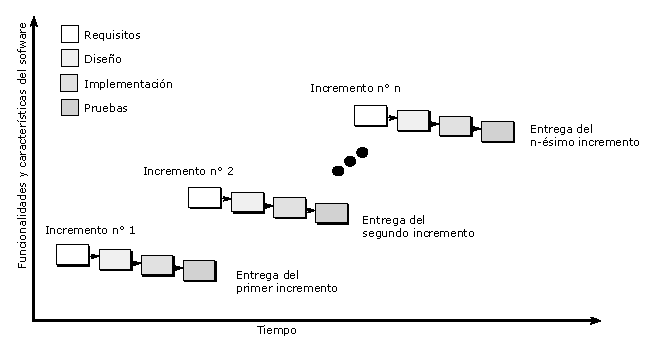
\includegraphics[width=\textwidth]{assets/iedevelopment-v2.eps}
                % \caption{caption}
                % \label{label}
            \end{figure}
        \end{columns}
    
    \end{frame}

    \subsection{Adaptaciones realizadas a la metodología}
    \begin{frame}
        \frametitle{Iterativa e incremental}            
        Adaptaciones realizadas a la metodología
        \begin{itemize}
            \item Disminuir la cantidad de documentación de cada fase
            \item Llevar a cabo más de una fase en una iteración al mismo tiempo
            \item Los roles de analista, diseñador, implementador y tester son llevado a cabo por una sola persona.
        \end{itemize}
    \end{frame}

    \section{Desarrollo}

    \subsection{Concepción del proyecto y planificación del proyecto}
    \begin{frame}
        \frametitle{Concepción del proyecto}                 
        \begin{itemize}
            \item Propuesta por parte del profesor Daniel Mora
            \item Proyecto Optimization of real-world water distribution systems and hydraulic elements using computational fluid dynamics (cfd) and evolutionary algorithms
            \item Jmetal + EpanetToolkit
        \end{itemize}
    \end{frame}

    \begin{frame}
        \frametitle{Planificación}                 
        \begin{itemize}
            \item \textbf{Iteración 1:} Requisitos y Arquitectura
            \item \textbf{Iteración 2:} Problema monoobjetivo y Algoritmo Genético (GA)
            \item \textbf{Iteración 3:} Interfaz gráfica (GUI)
            \item \textbf{Iteración 4:} Problema multiobjetivo y Algoritmo Non-Dominated Sorting Genetic Algorithm II (NSGAII)
            \item \textbf{Iteración 5:} Experimentos y simulación hidraúlica.
            \item \textbf{Iteración 6:} Afinación de detalles.
        \end{itemize}
    \end{frame}

    % \subsection{Tecnología utilizada}
    \begin{frame}
        \frametitle{Tecnología utilizada}                 
        \begin{columns}
            \column{0.33\textwidth}
            \begin{figure}[H]
                \centering
                
\includegraphics[width=\textwidth]{assets/Tecnologia/Java.png}
            \end{figure}

            \column{0.33\textwidth}
            \begin{figure}[H]
                \centering
                
\includegraphics[width=\textwidth]{assets/Tecnologia/JavaFX.png}
            \end{figure}

            \column{0.33\textwidth}
            \begin{figure}[H]
                \centering
                
\includegraphics[width=\textwidth]{assets/Tecnologia/EpanetToolkit.png}
            \end{figure}
        \end{columns}
    \end{frame}

    \subsection{Requisitos}
    \begin{frame}
        \frametitle{Requisitos}                 
        
        \begin{itemize}
            \item Captura, priorización y especificación formal de los requisitos
            \item 32 Requisitos de usuario
            \item Documento de especificación formal de requisitos.
        \end{itemize}

        \begin{figure}
            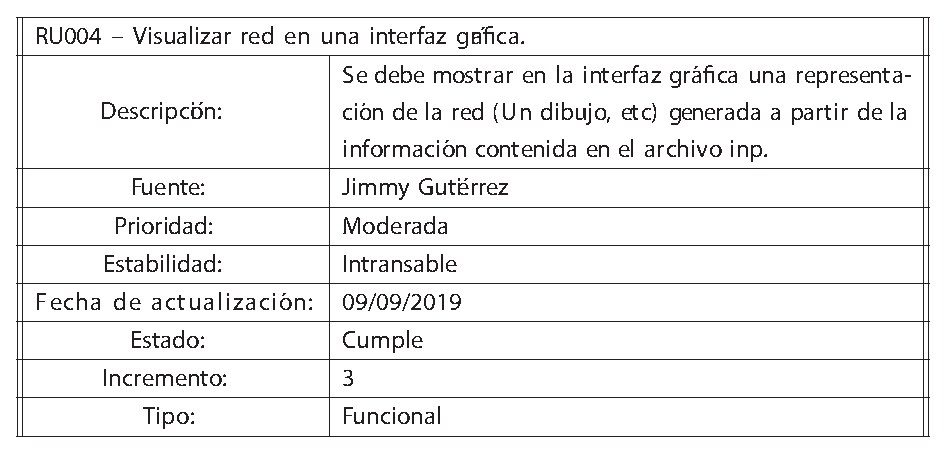
\includegraphics[width=0.8\textwidth]{assets/Requisito.eps}
        \end{figure}

    \end{frame}

    \subsection{Diseño}
    \begin{frame}
        \frametitle{Diseño}                 
                
        \begin{itemize}
            \item Diseñar los módulos de la aplicación y la interacción entre ellos.
            \item Documento de diseño
            
            \begin{itemize}
                \item Arquitectura Física
                \item Arquitectura Lógica
                \item Diagrama de clases
                \item Diagrama de secuencia
                \item Diseño de interfaces
            \end{itemize}
        \end{itemize}

    \end{frame}

    \begin{frame}
        \frametitle{Arquitectura Fisica}                       
        Monolítica
        \begin{figure}
            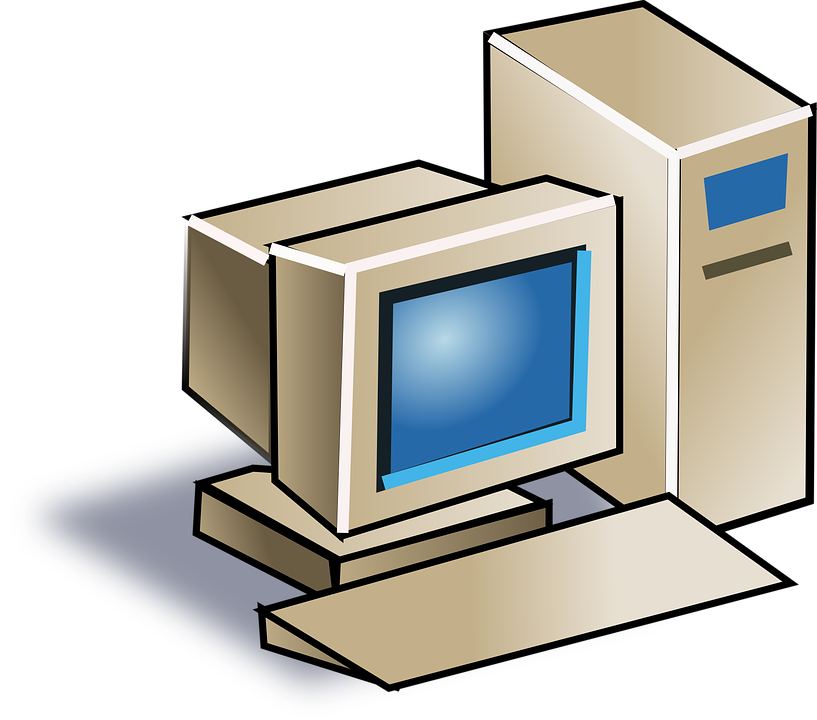
\includegraphics[width=0.5\textwidth]{assets/ArquitecturaFisica.png}
        \end{figure}

    \end{frame}

    \begin{frame}
        \frametitle{Arquitectura Lógica}  

        Modelo-Vista-Controlador
        \begin{figure}
            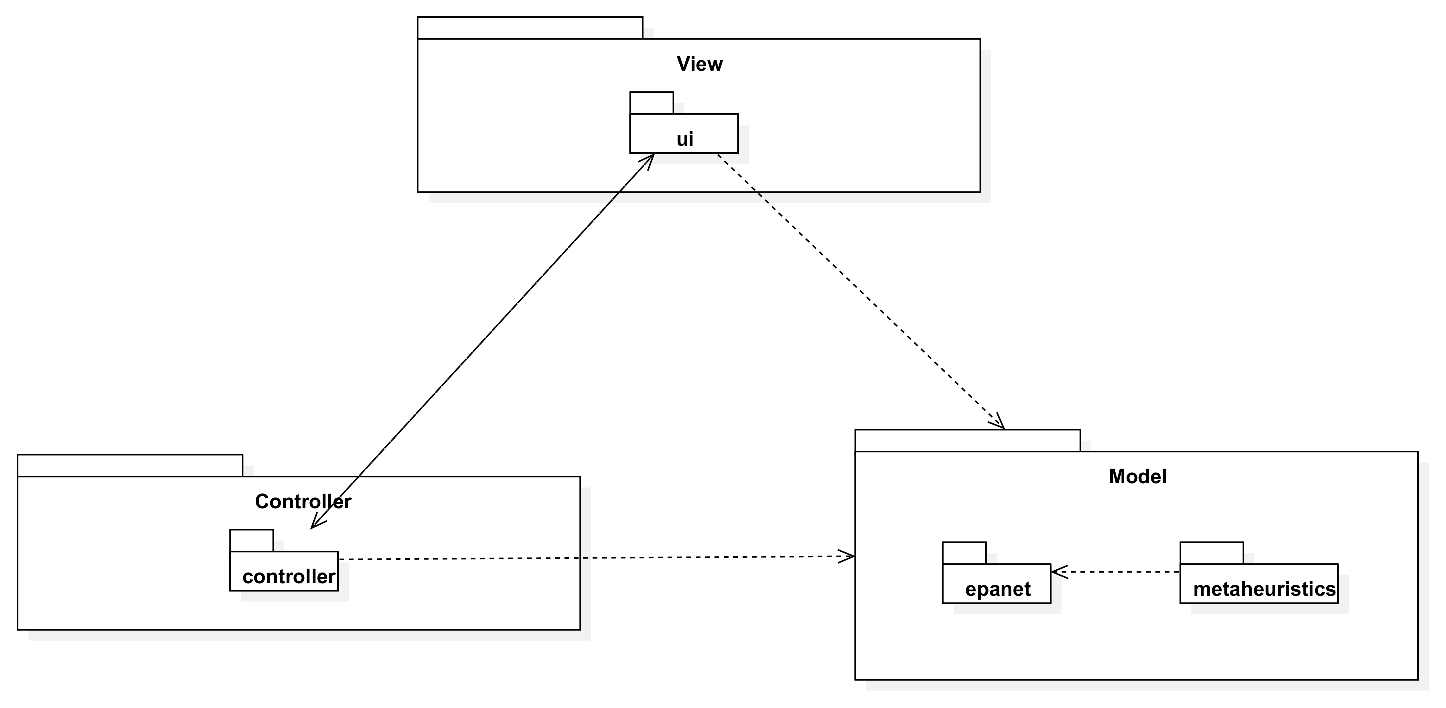
\includegraphics[width=0.8\textwidth]{assets/ArquitecturaLogica.eps}
        \end{figure}

    \end{frame}

    \subsection{Implementación}

    \begin{frame}
        \frametitle{Implementación}                       
        Codificación y generación del manual de usuario.

    \end{frame}

    \begin{frame}
        \frametitle{Implementación}
        Ventana Principal                   
        \begin{figure}
            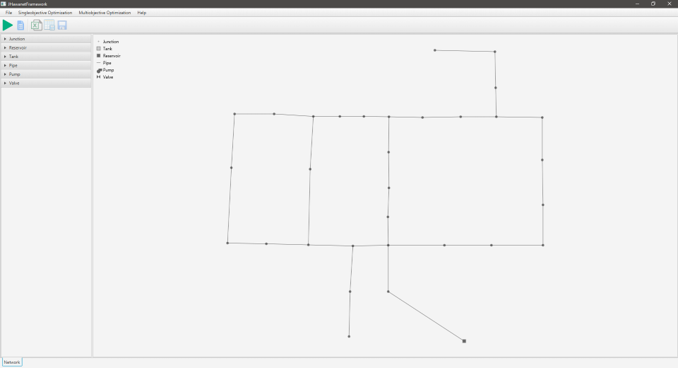
\includegraphics[width=\textwidth]{assets/Interfaces/Principal.png}
        \end{figure}
    \end{frame}
    
    \begin{frame}
        \frametitle{Implementación}
        Ventana de Configuración                
        
        \begin{columns}
            \column{0.5\textwidth}
            \begin{figure}
                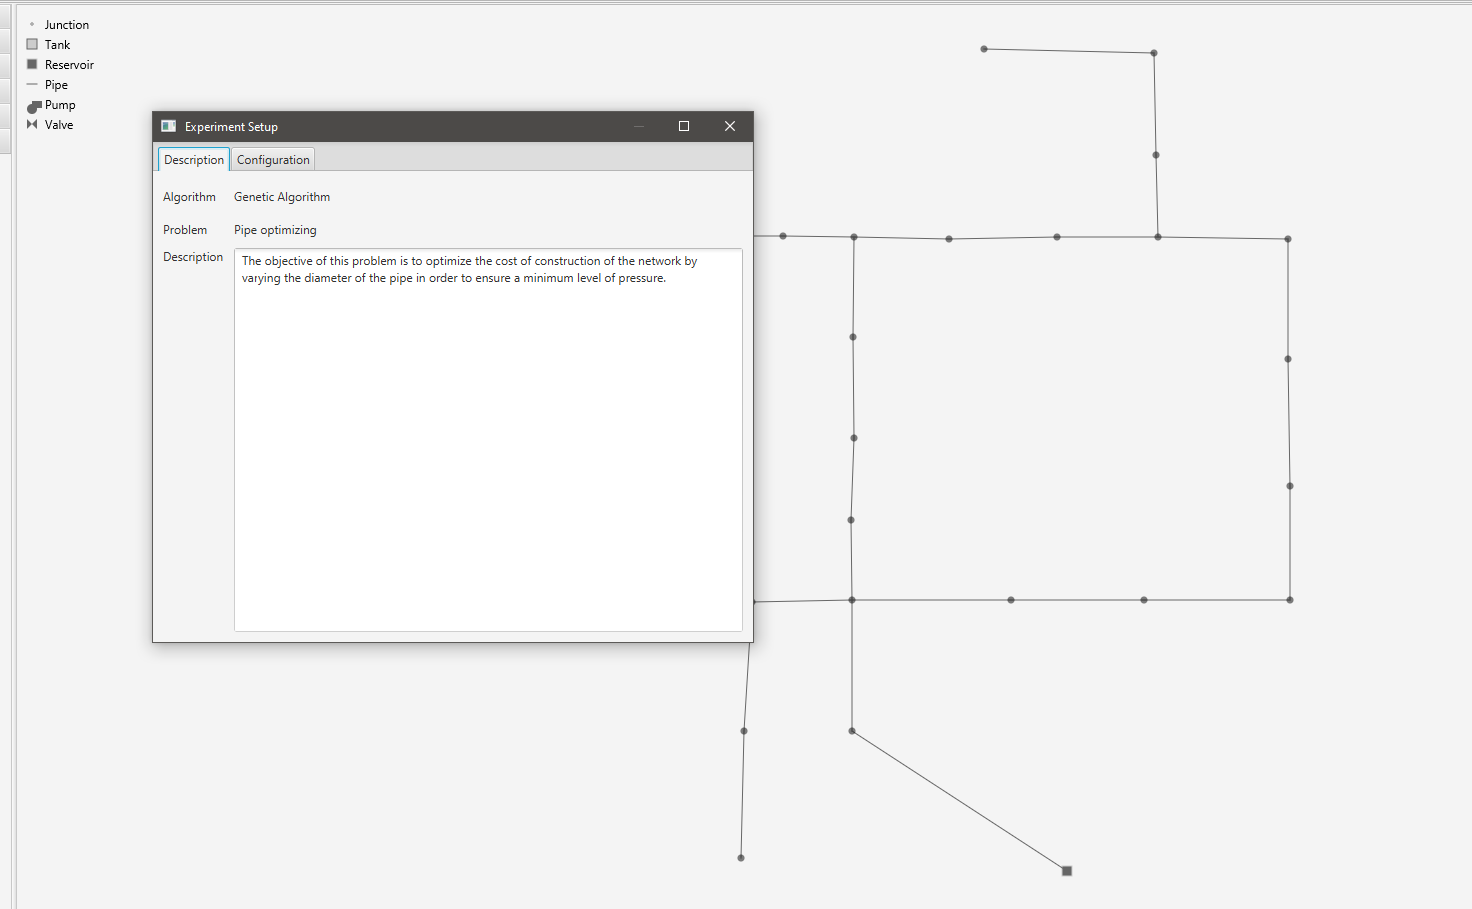
\includegraphics[width=\textwidth]{assets/Interfaces/ConfiguracionProblema1.png}
            \end{figure}
            \column{0.5\textwidth}
            \begin{figure}
                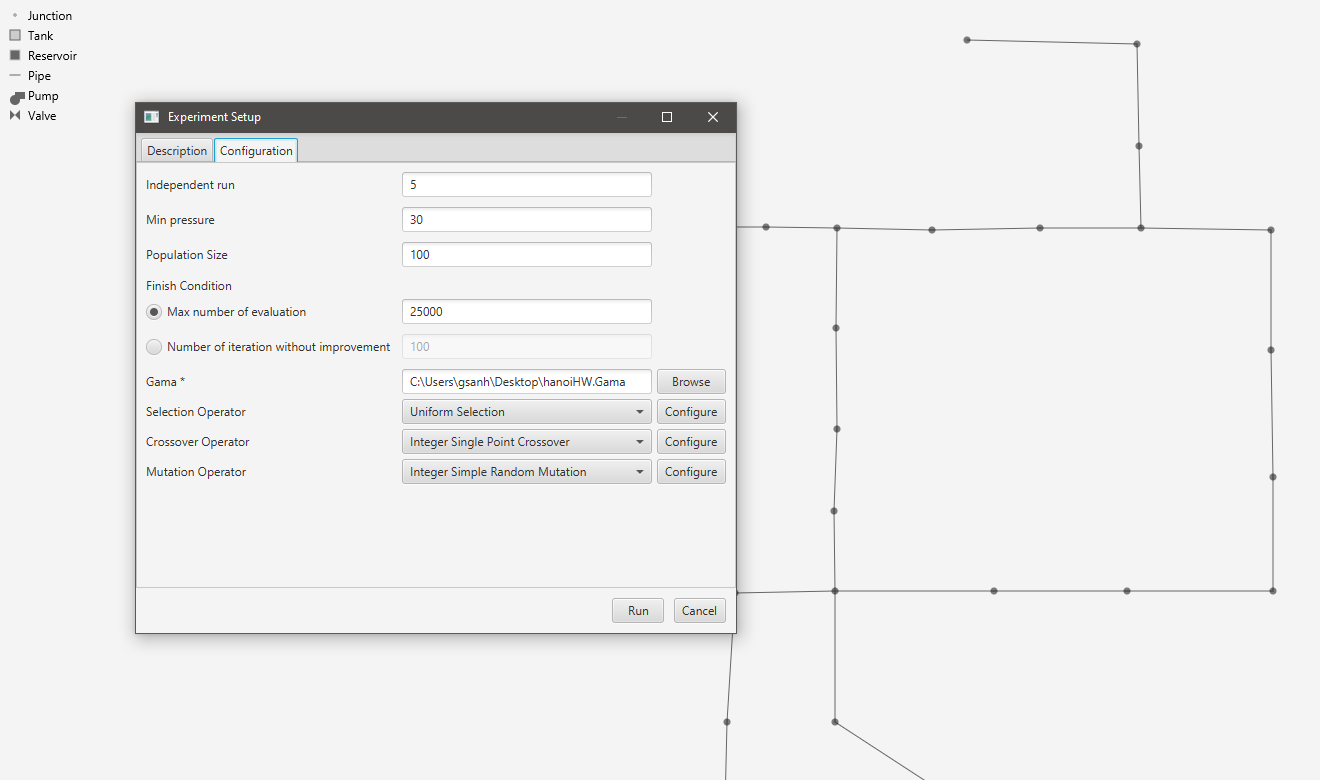
\includegraphics[width=\textwidth]{assets/Interfaces/ConfiguracionProblema2.png}
            \end{figure}
        \end{columns}
    \end{frame}
    
    \begin{frame}
        \frametitle{Implementación}
        Ventana de ejecución               
        \begin{figure}
            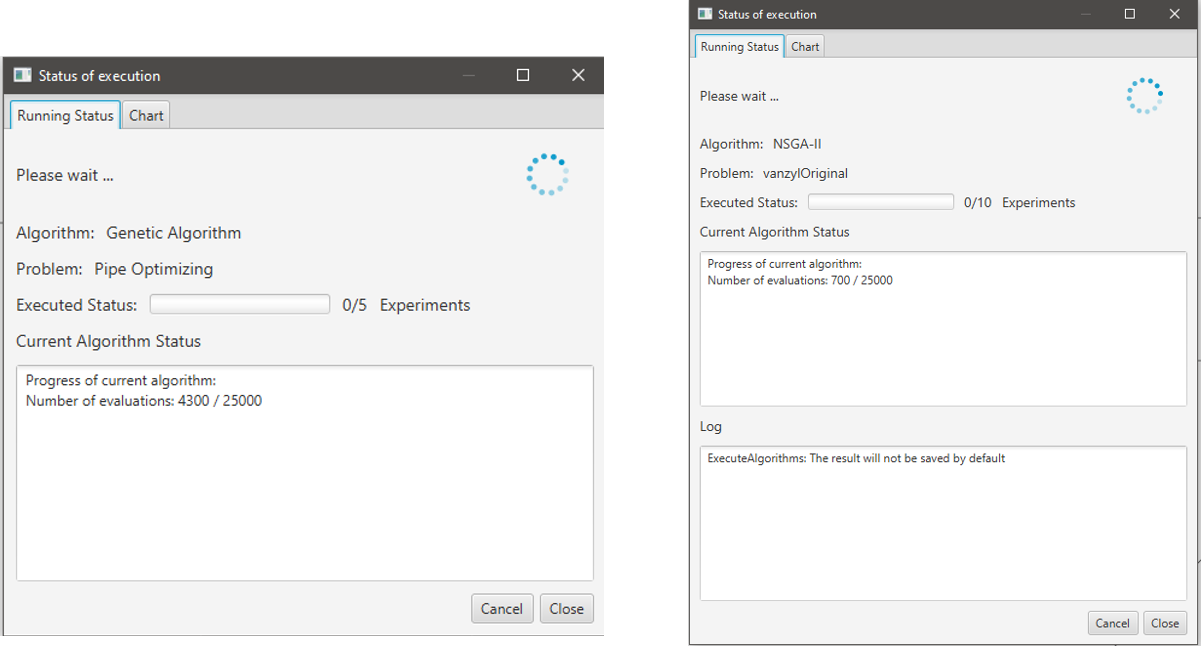
\includegraphics[width=\textwidth]{assets/Interfaces/EstadoEjecucion.png}
        \end{figure}
    \end{frame}

    \begin{frame}
        \frametitle{Implementación}
        Gráfico de resultados                  
        \begin{figure}
            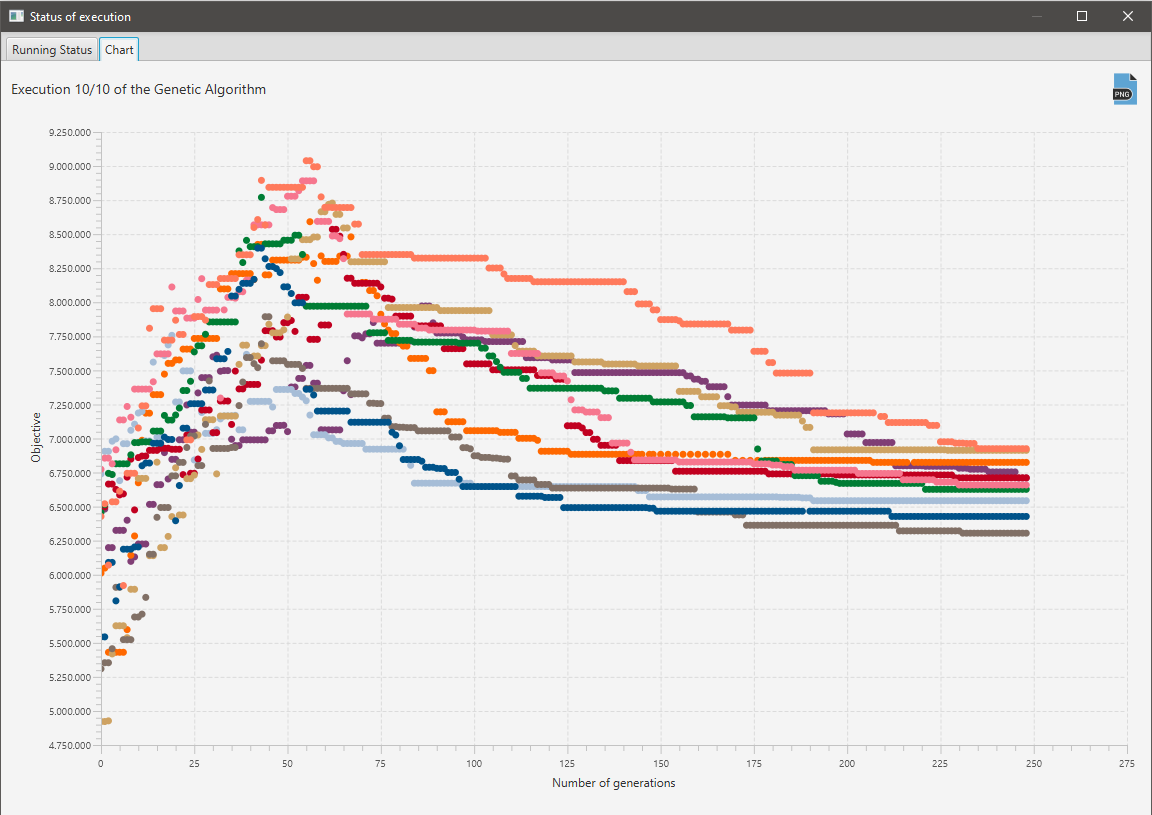
\includegraphics[width=0.75\textwidth]{assets/Interfaces/GraficoResultados.png}
        \end{figure}
    \end{frame}

    \begin{frame}
        \frametitle{Implementación}
        Resultados Optimización                
        \begin{figure}
            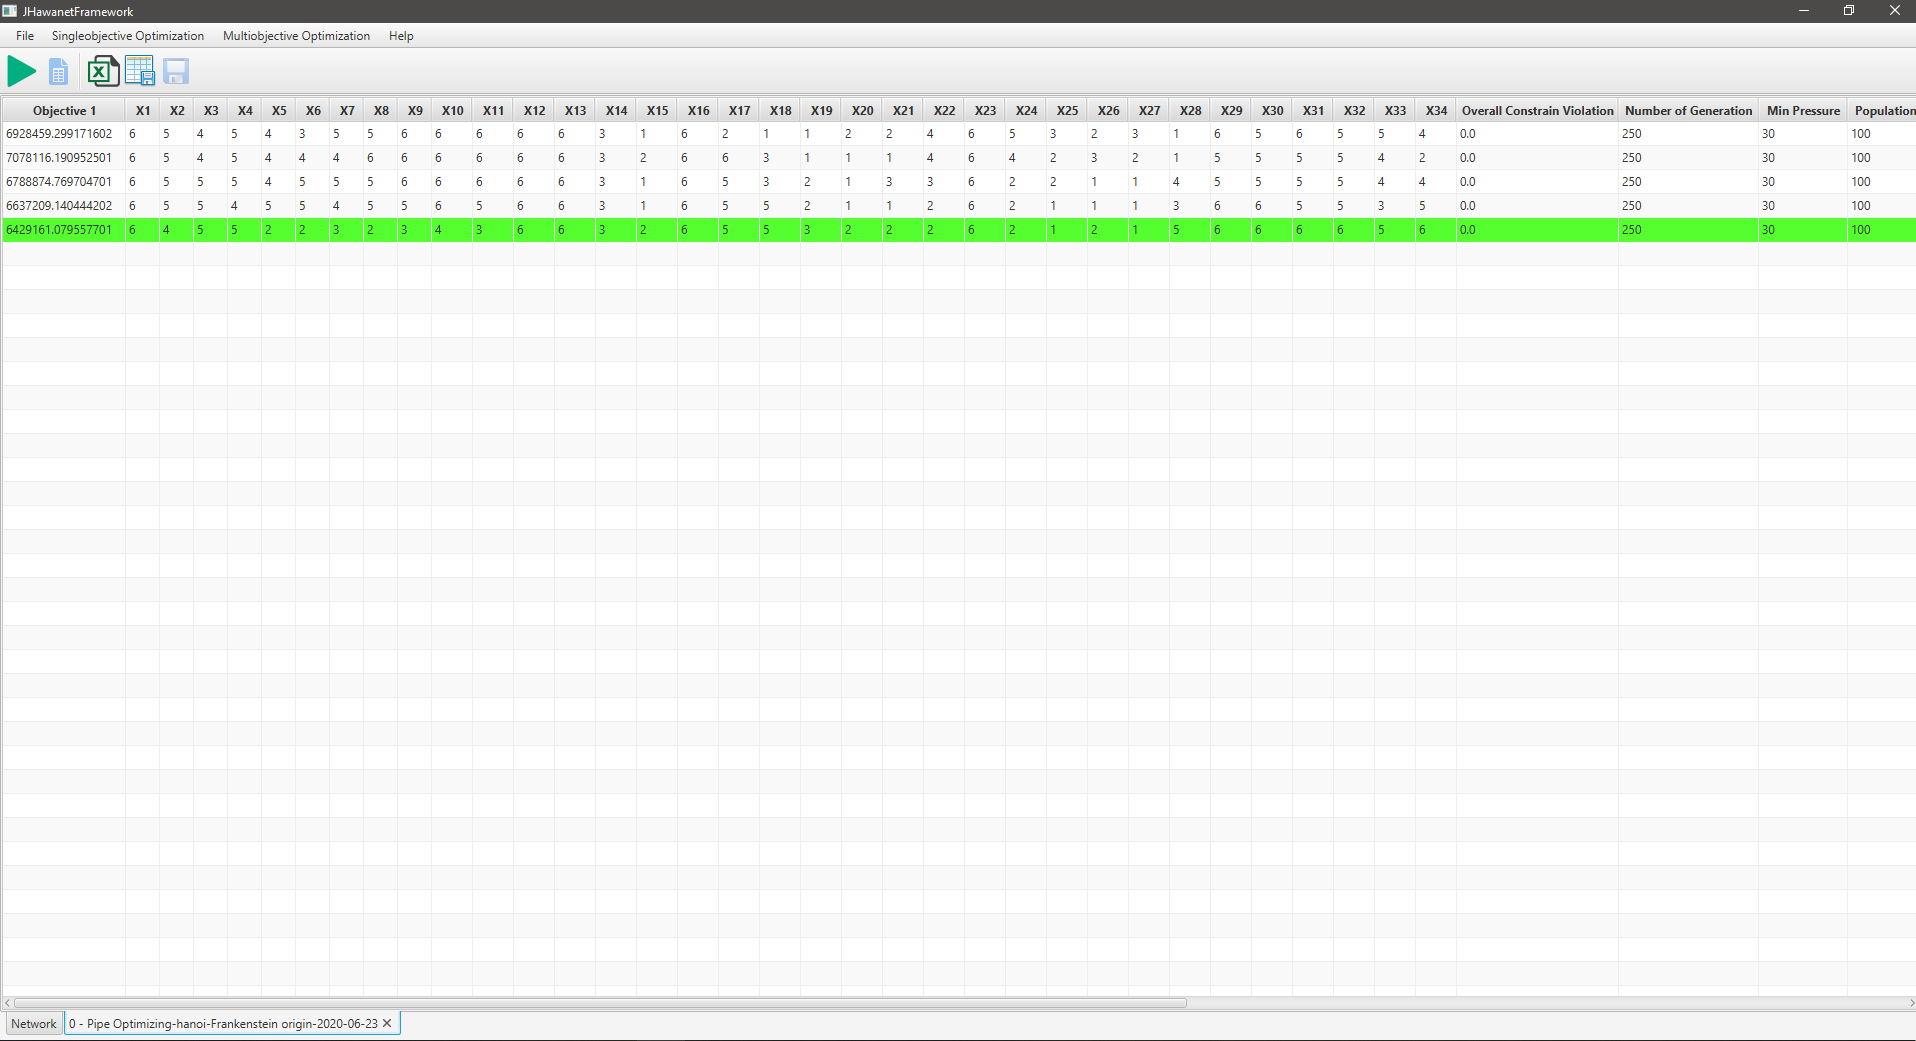
\includegraphics[width=\textwidth]{assets/Interfaces/Resultados.png}
        \end{figure}
    \end{frame}

    \begin{frame}
        \frametitle{Implementación}
        Ventana de simulación hidráulica                 
        \begin{figure}
            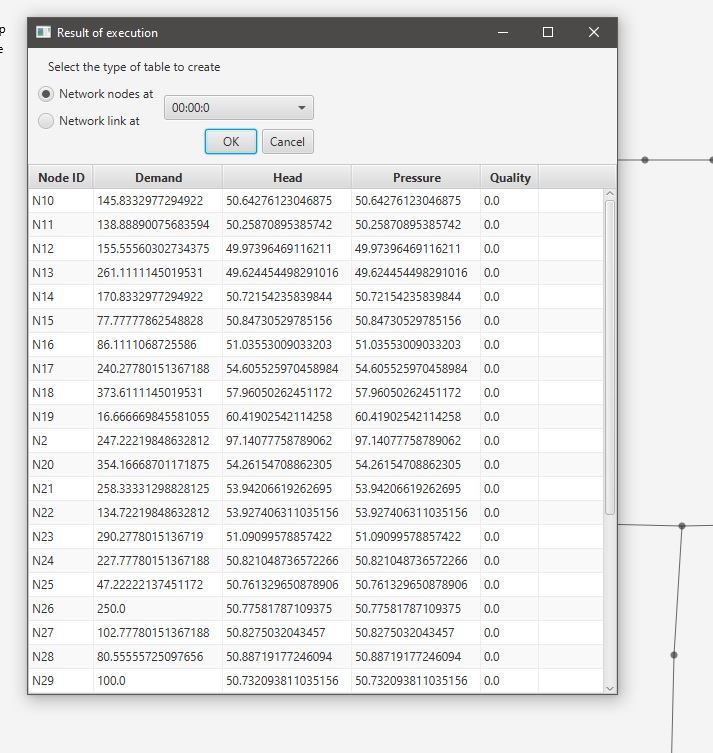
\includegraphics[height=0.8\textheight]{assets/Interfaces/ResultadosSimulacion.png}
        \end{figure}
    \end{frame}

    \begin{frame}
        \frametitle{Implementación}                       
        \textit{Java Reflection} y \textit{Java Annotation}
        \begin{figure}
            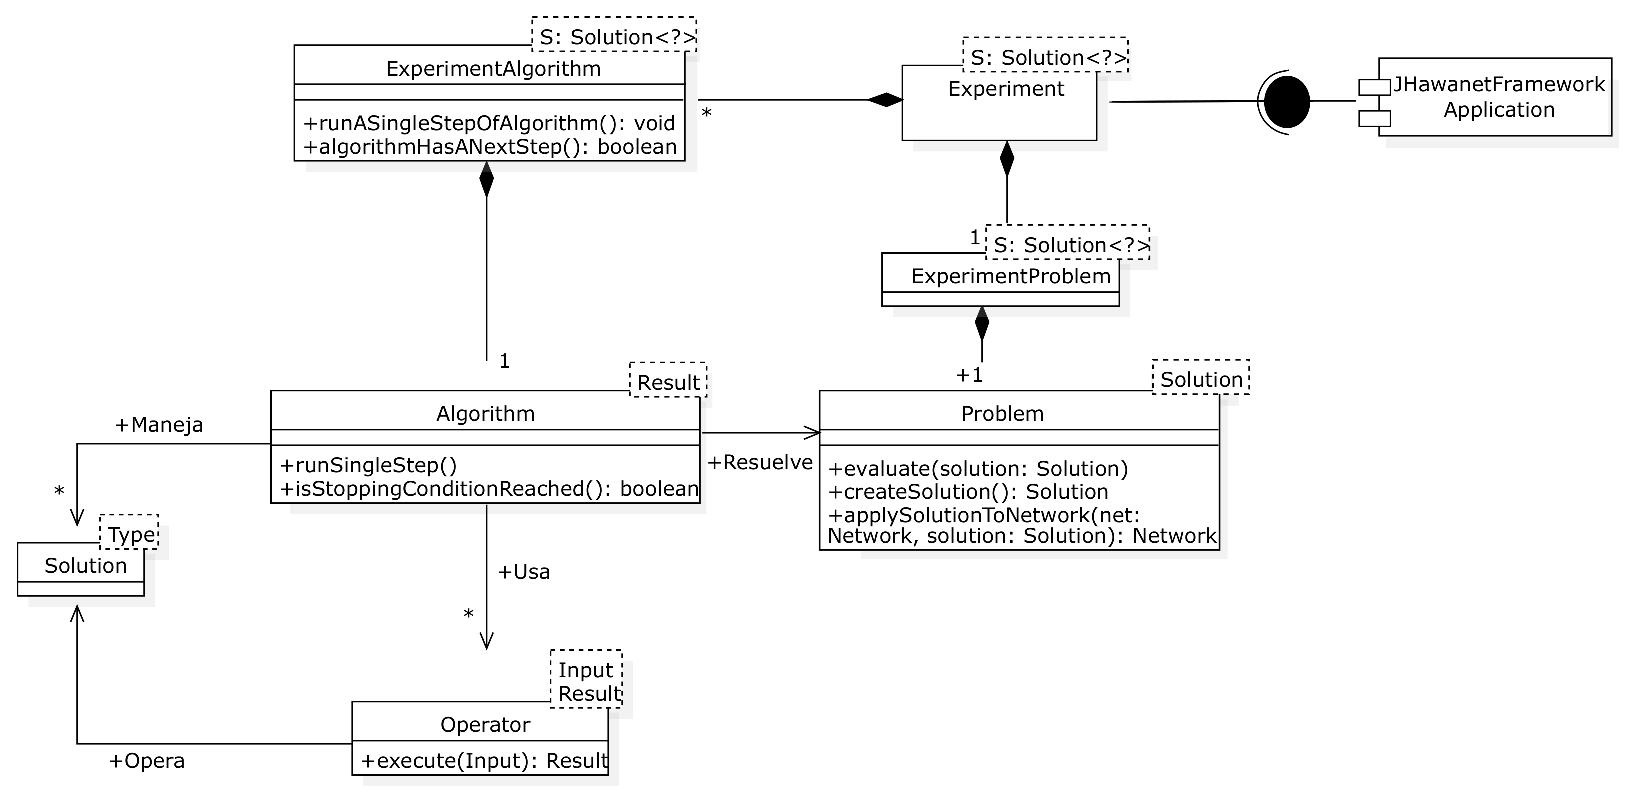
\includegraphics[width=\textwidth]{assets/InterfazHumano-app.eps}
        \end{figure}

    \end{frame}

    \begin{frame}
        \frametitle{Implementación}                       
        \begin{itemize}
            \item Problema de diseño de RDA basado en el costo de tuberías
        \end{itemize} 

        \begin{block}{Objetivo}
            \begin{equation*}
                \text{Costo de inversión} = \sum_{i=1}^{N} (C_i \times D_i \times L_i)
            \end{equation*}
        \end{block}
        
    \end{frame}

    \begin{frame}
        \frametitle{Implementación}                       
        Problema de operación basado en el Régimen de bombeo
        
        \begin{block}{Objetivo 1}
            \begin{equation*}
                C_E(S) = \sum_{n=1}^{NP}\sum_{t=0}^{NT-1}(P_c(t) \times E_c(n, t) \times S(n, t))
            \end{equation*}
        \end{block}

        \begin{block}{Consumo energético}
            \begin{equation*}
                E_c(n, t) = \frac{10^{-3} \times \gamma \times Q(n, t) \times h(n, t)}{e(n, t)}
            \end{equation*}
        \end{block}
        
        \begin{block}{Objetivo 2}
            \begin{equation*}
                C_N(S) = \sum_{n=1}^{NP}\sum_{t=0}^{NT-1}r_t
            \end{equation*}
        \end{block}
    \end{frame}

    \begin{frame}
        \frametitle{Implementación}                       
        Algoritmo Genético

        \begin{figure}
            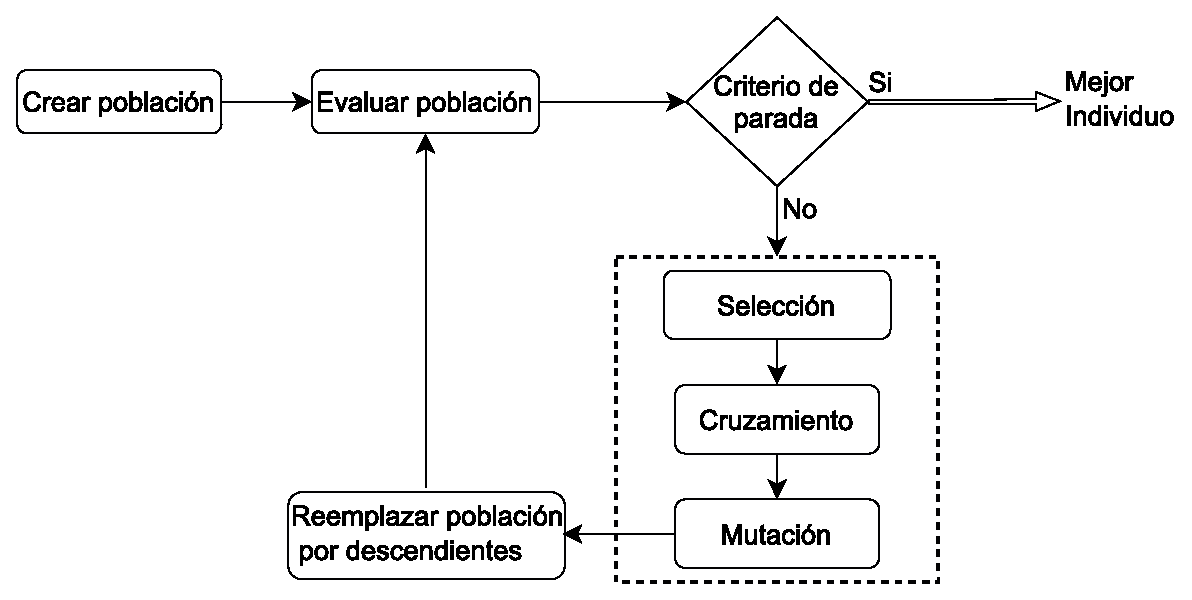
\includegraphics[width=0.8\textwidth]{assets/AlgoritmoGenetico.eps}
        \end{figure}

    \end{frame}

    \begin{frame}
        \frametitle{Implementación}                       
        Non-dominated Sorting Genetic Algorithm-II (INSGA-II)

        \begin{figure}
            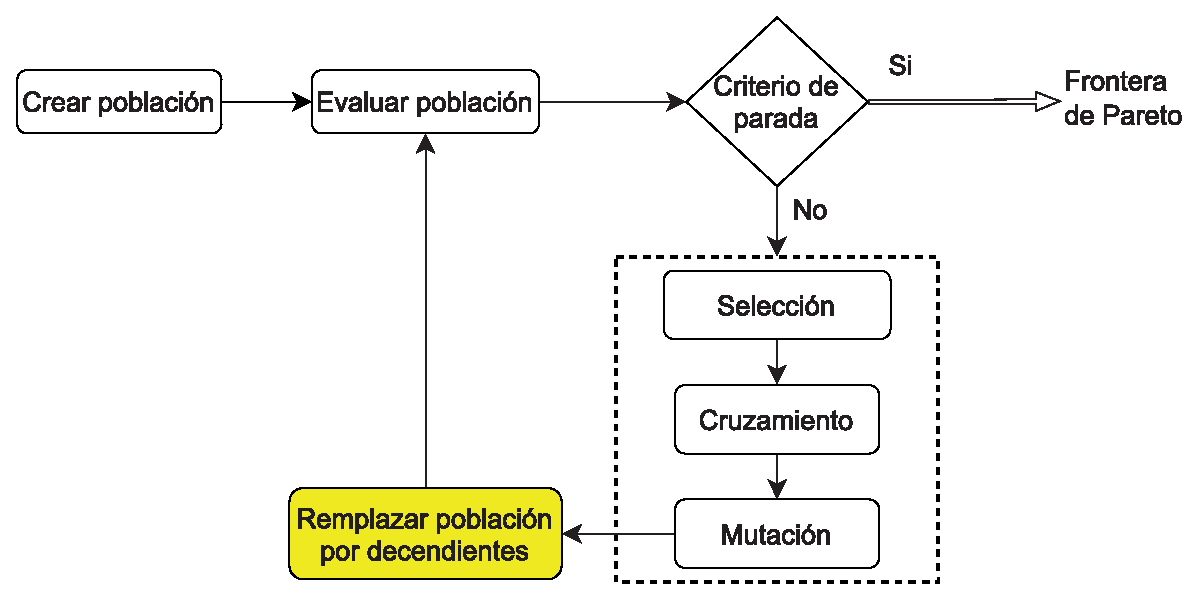
\includegraphics[width=0.8\textwidth]{assets/NSGAIIFlujo.eps}
        \end{figure}

    \end{frame}

    \begin{frame}
        \frametitle{Implementación}                       
        Non-dominated Sorting Genetic Algorithm-II (INSGA-II)

        \begin{figure}
            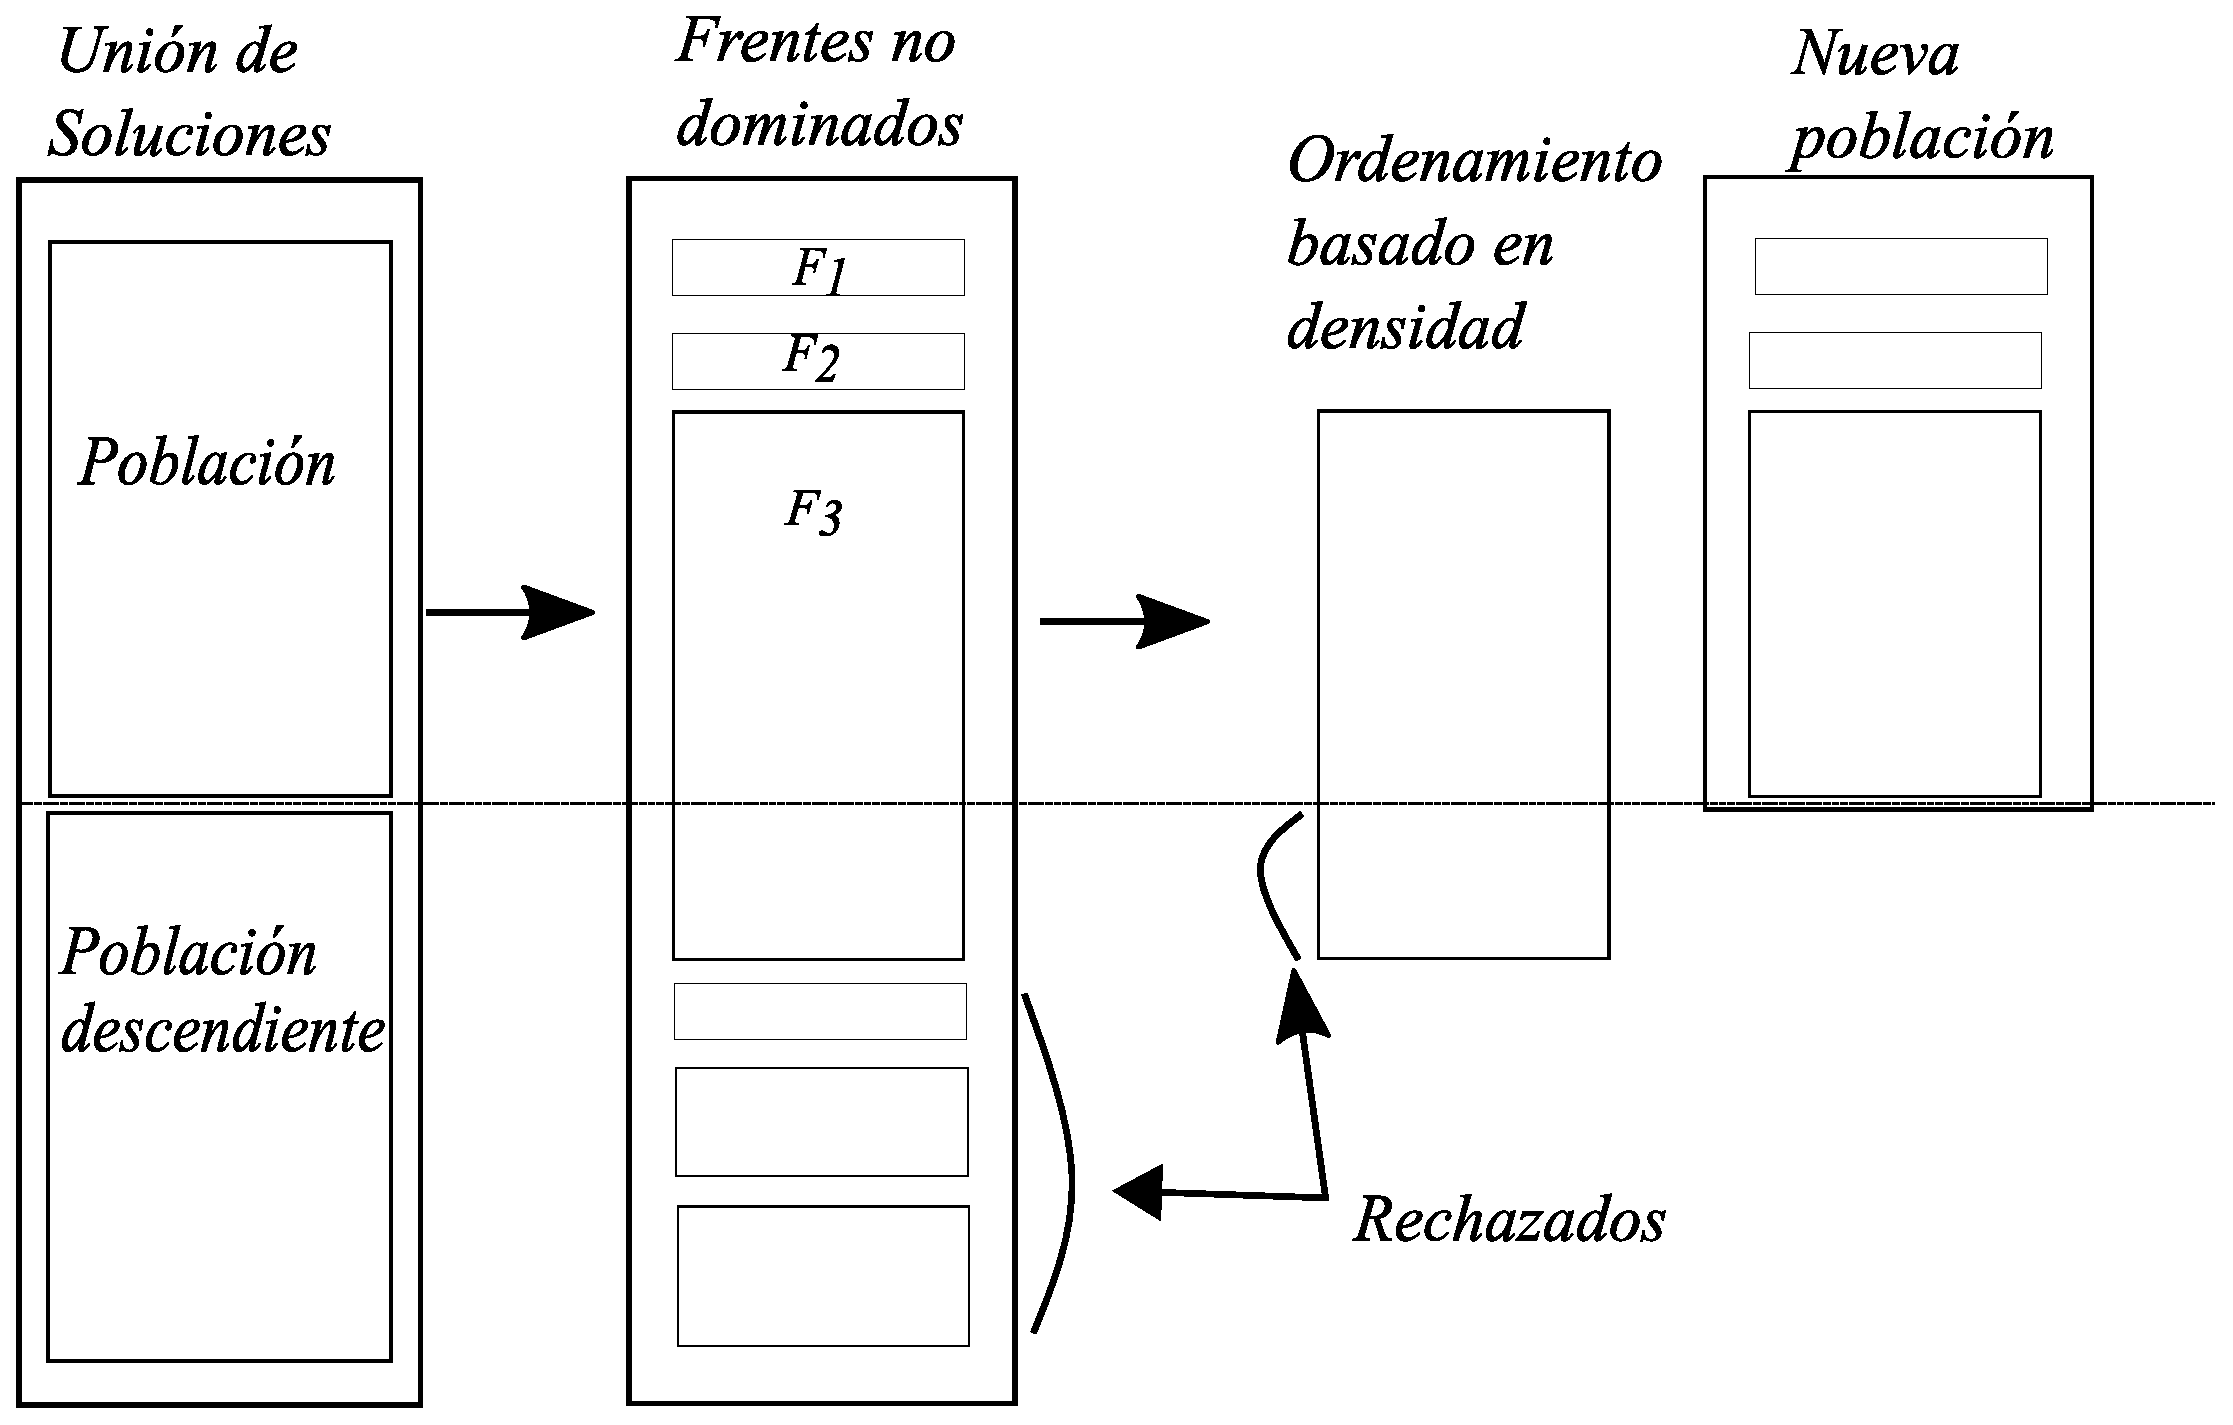
\includegraphics[width=0.8\textwidth]{assets/NSGAII.eps}
        \end{figure}

    \end{frame}

    \subsection{Pruebas}
    \begin{frame}
        \frametitle{Pruebas}                       
        
        \begin{itemize}
            \item Realización de pruebas y su especificación formal
            \item 39 Pruebas automatizadas
            \item 16 Pruebas manuales
            \item Documento de especificación formal de pruebas
        \end{itemize}


    \end{frame}

    \begin{frame}
        \frametitle{Pruebas}     
        Prueba Automatizada
        \begin{figure}
            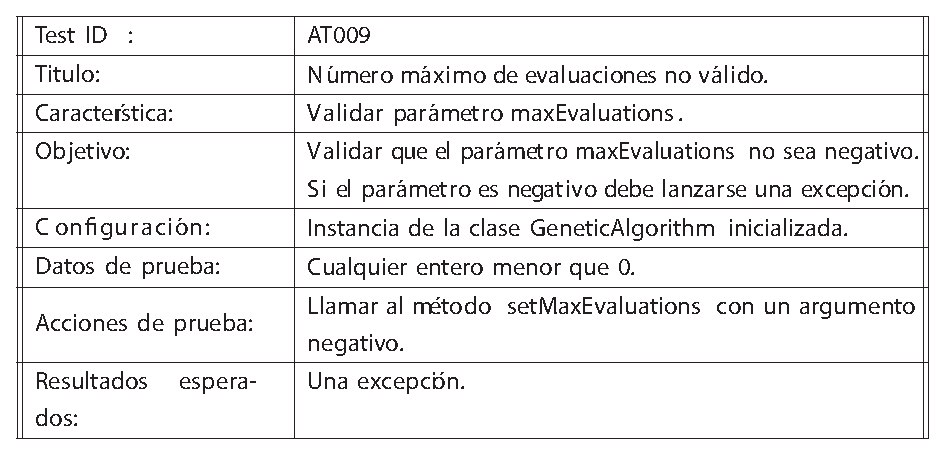
\includegraphics[width=0.8\textwidth]{assets/PruebaAutomatizada.eps}
        \end{figure}
        
    \end{frame}

    \begin{frame}
        \frametitle{Pruebas}     
        Prueba Manual
        \begin{figure}
            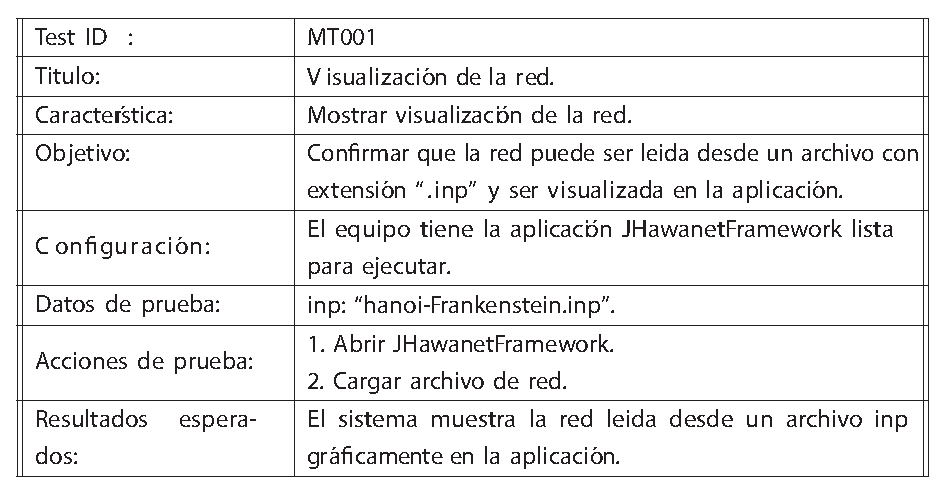
\includegraphics[width=0.8\textwidth]{assets/PruebaManual.eps}
        \end{figure}
        
    \end{frame}

    \section{Evaluación}
    \subsection{Diseño del caso}

    \begin{frame}
        \frametitle{Diseño del caso}                       
        
        \begin{itemize}
            \item Elección del caso
            \begin{itemize}
                \item La aplicación desarrollada
            \end{itemize}

            \item Objetivos de la investigación
            \begin{itemize}
                \item ¿Cómo el sistema desarrollado trabaja en la práctica?
            \end{itemize}

            \item Características a evaluar
            \begin{itemize}
                \item Funcionalidad
                \item Usabilidad
                \item Utilidad
                \item Utilidad del manual de usuario
            \end{itemize}
        \end{itemize}

    \end{frame}

    \begin{frame}
        \frametitle{Diseño del caso}                       
        
        \begin{itemize}
            \item Protocolo para conducir el estudio de caso
            \item Unidad de análisis
            \begin{itemize}
                \item Profesionales con conocimientos en computación, hidráulica y metaheurísticas
            \end{itemize}

            \item Consideraciones técnicas	  
            \begin{itemize}
                \item Window 64bits
                \item Java 1.8
            \end{itemize}

            \item Consideraciones para los usuarios
            \begin{itemize}
                \item Conocimientos básicos en hidráulica y metaheurísticas para saber interpretar los resultados de la aplicación. Si se desea incorporar nuevos algoritmos debe tener conocimientos en programación.
        
            \end{itemize}
        \end{itemize}

    \end{frame}

    \subsection{Recolección de datos}
    \begin{frame}
        \frametitle{Recolección de datos}                       
        
        
        \begin{itemize}
            \item Participantes
            \begin{itemize}
                \item Yamisleydi Salgueiro
                \item Marco Alsina
                \item Sergio Silva
            \end{itemize}

            \item Instrumentos para la recolección de los datos
            \begin{itemize}
                \item Encuesta utilizando la escala de Likert
                \item Test de usabilidad SUS
            \end{itemize}
        \end{itemize}

    \end{frame}

    \subsection{Análisis de datos}
    \begin{frame}      
        \frametitle{Análisis de datos}
        \begin{figure}
            \centering
            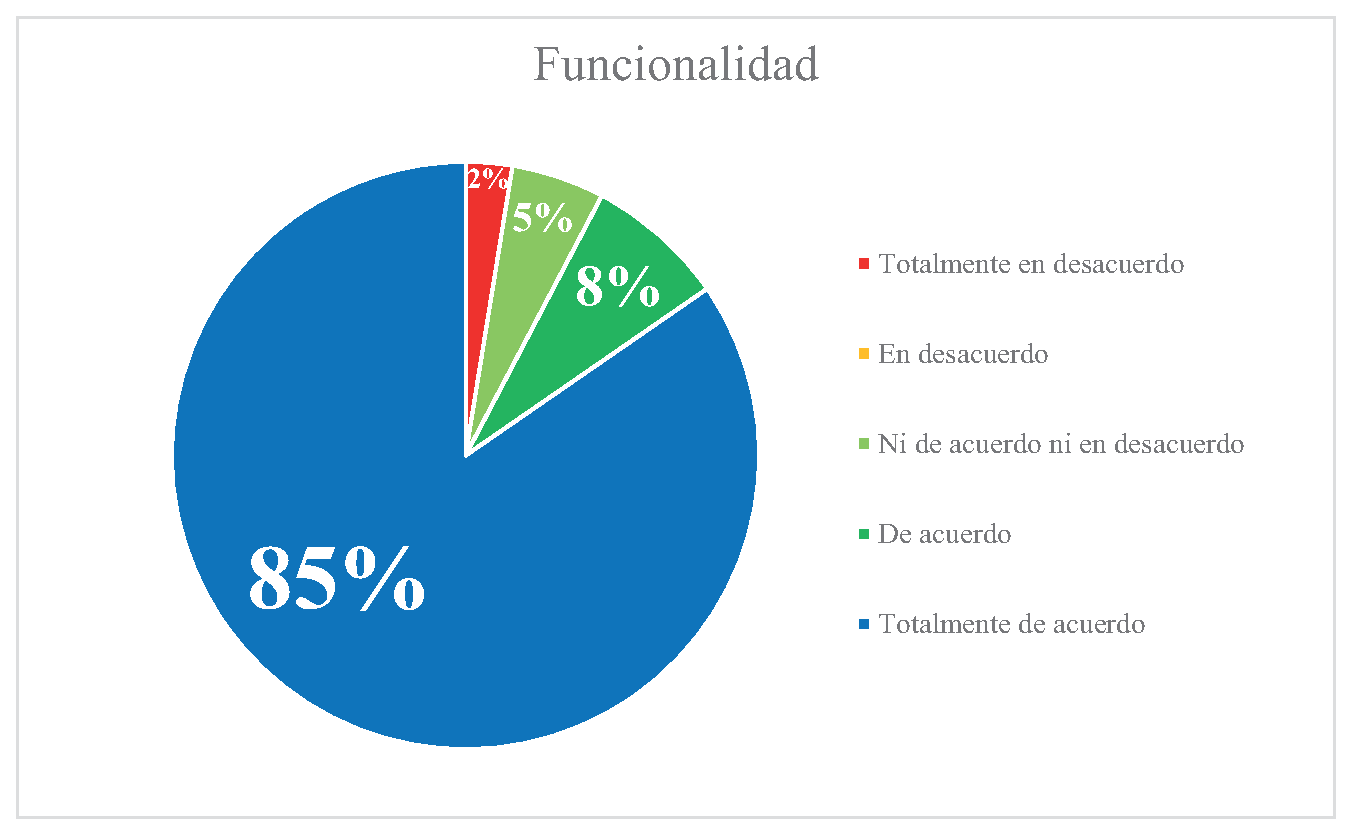
\includegraphics[width=0.9\textwidth]{assets/Evaluacion/funcionality.eps}
            % \caption{Gráfico circular de los resultados de la evaluación de funcionalidad de la aplicación}
        \end{figure}
    \end{frame}

    \begin{frame}      
        \frametitle{Análisis de datos}
       
       \begin{columns}
            \column{0.4\textwidth}
            $$ \bar{x}_{SUS} = 79.17$$
            $$ s_{SUS} = 9.46$$
    
            \column{0.6\textwidth}
            \begin{figure}
                \centering
                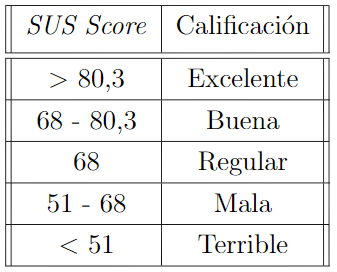
\includegraphics[width=\textwidth]{assets/Evaluacion/SUS_Score.png}
                % \caption{Gráfico circular de los resultados de la evaluación de funcionalidad de la aplicación}
            \end{figure}
       \end{columns}
    \end{frame}

    \begin{frame}      
        \frametitle{Análisis de datos}
        \begin{figure}
            \centering
            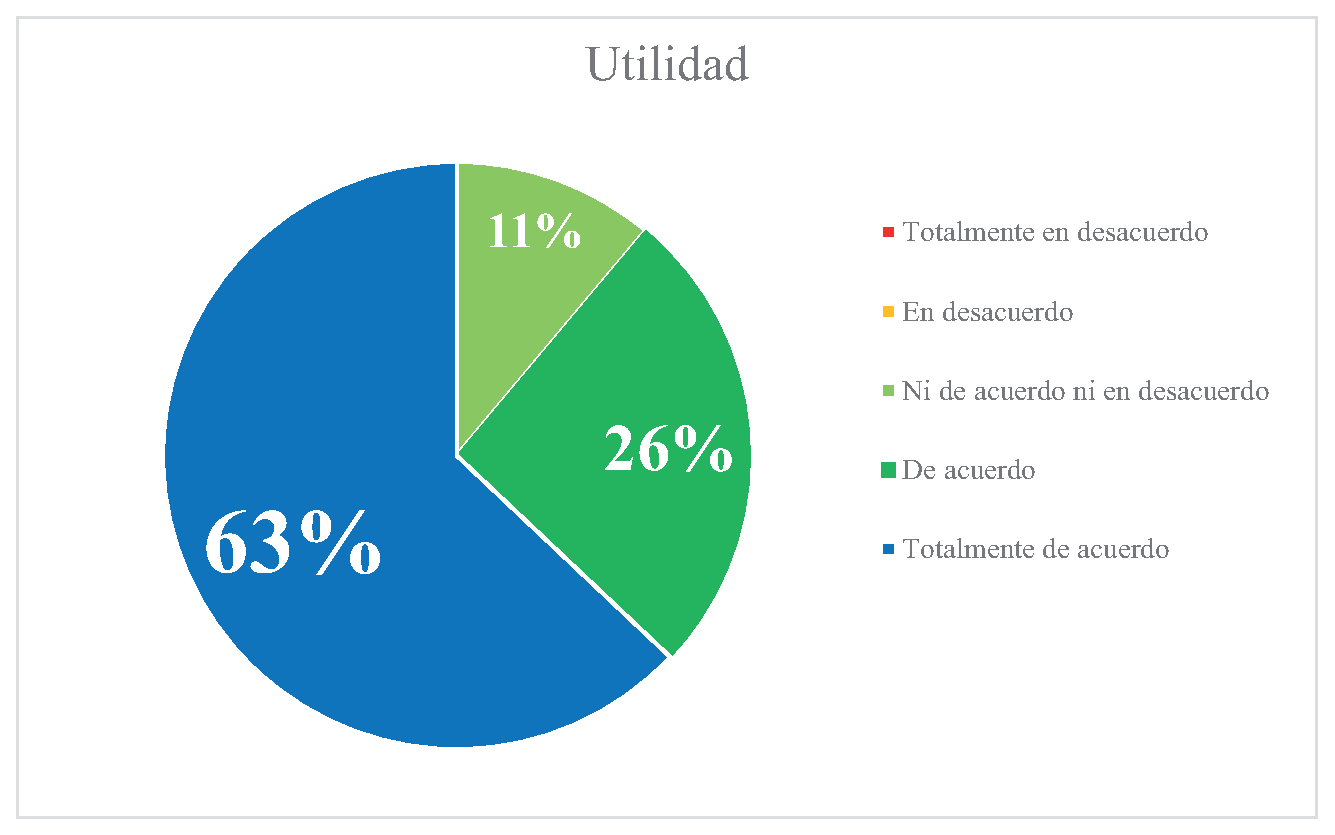
\includegraphics[width=0.9\textwidth]{assets/Evaluacion/utility.eps}
            % \caption{Gráfico circular de los resultados de la evaluación de funcionalidad de la aplicación}
        \end{figure}
    \end{frame}

    \begin{frame}      
        \frametitle{Análisis de datos}
        \begin{figure}
            \centering
            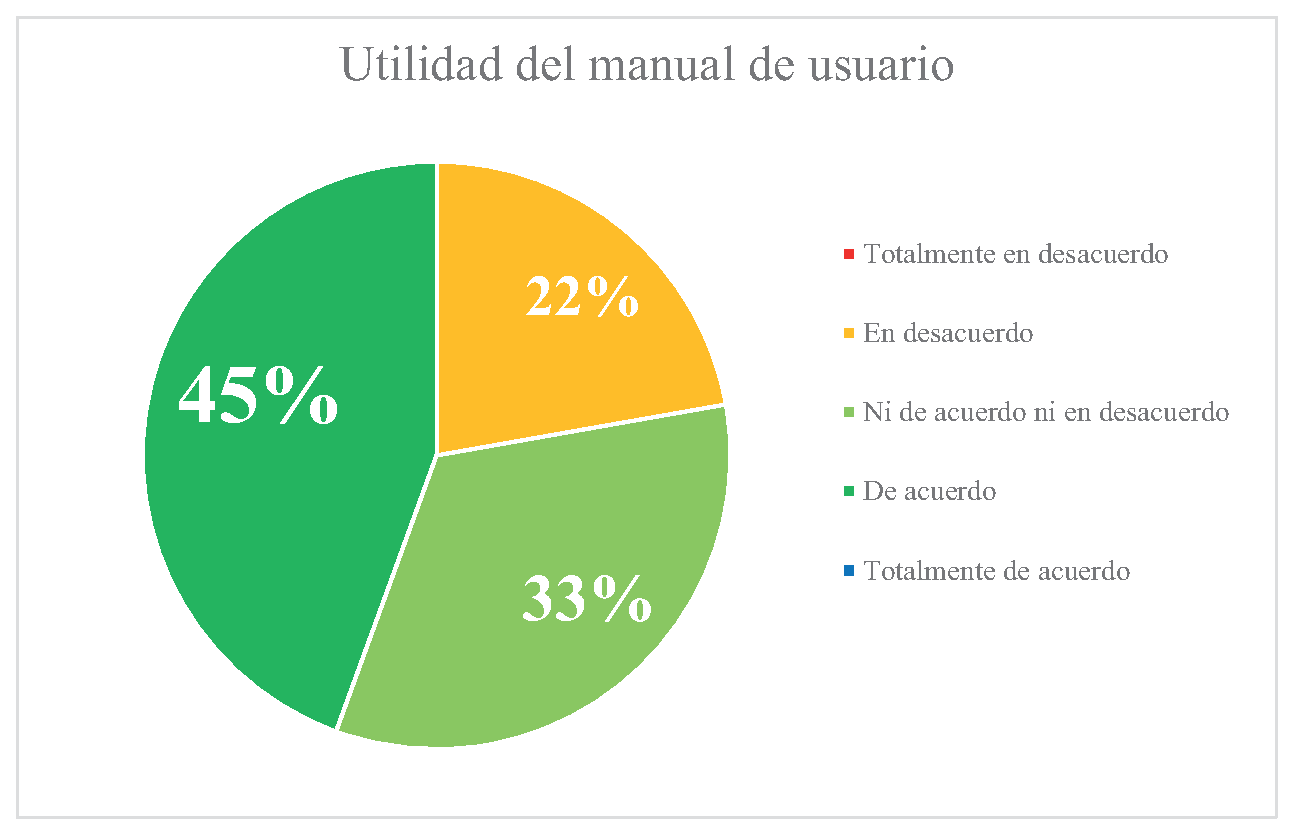
\includegraphics[width=0.9\textwidth]{assets/Evaluacion/manual_utility.eps}
            % \caption{Gráfico circular de los resultados de la evaluación de funcionalidad de la aplicación}
        \end{figure}
    \end{frame}

    \subsection{Conclusiones estudio de caso}
    \begin{frame}      
        \frametitle{Conclusiones estudio de caso}
        
        \begin{itemize}
            \item Criterios de funcionalidad, usabilidad y utilidad cumplidos, concluyendo que el sistema trabaja bien en la práctica. 
            \item Criterio de utilidad del manual de usuario no cumplido por lo que se deben realizar cambios para mejorar la información y ayuda que se entrega con éste.
        \end{itemize}
    \end{frame}

    \section{Conclusiones y Trabajos Futuros}
    \subsection{Conclusiones}
    \begin{frame}
        \frametitle{Conclusiones}                       
        
        \begin{itemize}
            \item Software para la optimización de los procesos de diseño y operación  de RDA.
            \item Todos los objetivos establecidos fueron logrados cumplidos
        \end{itemize}
    
    \end{frame}

    \subsection{Trabajos Futuros}
    \begin{frame}
        \frametitle{Trabajos Futuros}                       
           
        \begin{itemize}
            \item Agregar nuevos algoritmos, operadores y problemas
            \item Recortar el numero de decimales utilizados
            \item Permitir exportar la imagen de la red
            \item Guardar las imágenes exportadas en un formato vectorial
            \item Cambiar tamaño de los iconos cuando el cursor este encima
            \item Permitir agregar formulas LaTeX en la descripción del algoritmo
            \item Permitir utilizar distintos algoritmos en un mismo Experimento
            \item Añadir métricas de comparación entre algoritmos
            \item Añadir en el menú contextual los patrones de bombeo o demanda en caso de que la red cargada los especifique.
            \item Permitir resetear a los valores por defecto  en la ventana de configuración del problema
        \end{itemize}

    
    \end{frame}

    \begin{frame}    
        \centering       
        \Huge{Fin}
    \end{frame}

    \section{Anexo}
    \subsection{Operadores de Selección}
    \begin{frame}
        \frametitle{Operadores de Selección}                       
        \textit{Tournament Selection}
        \begin{figure}
            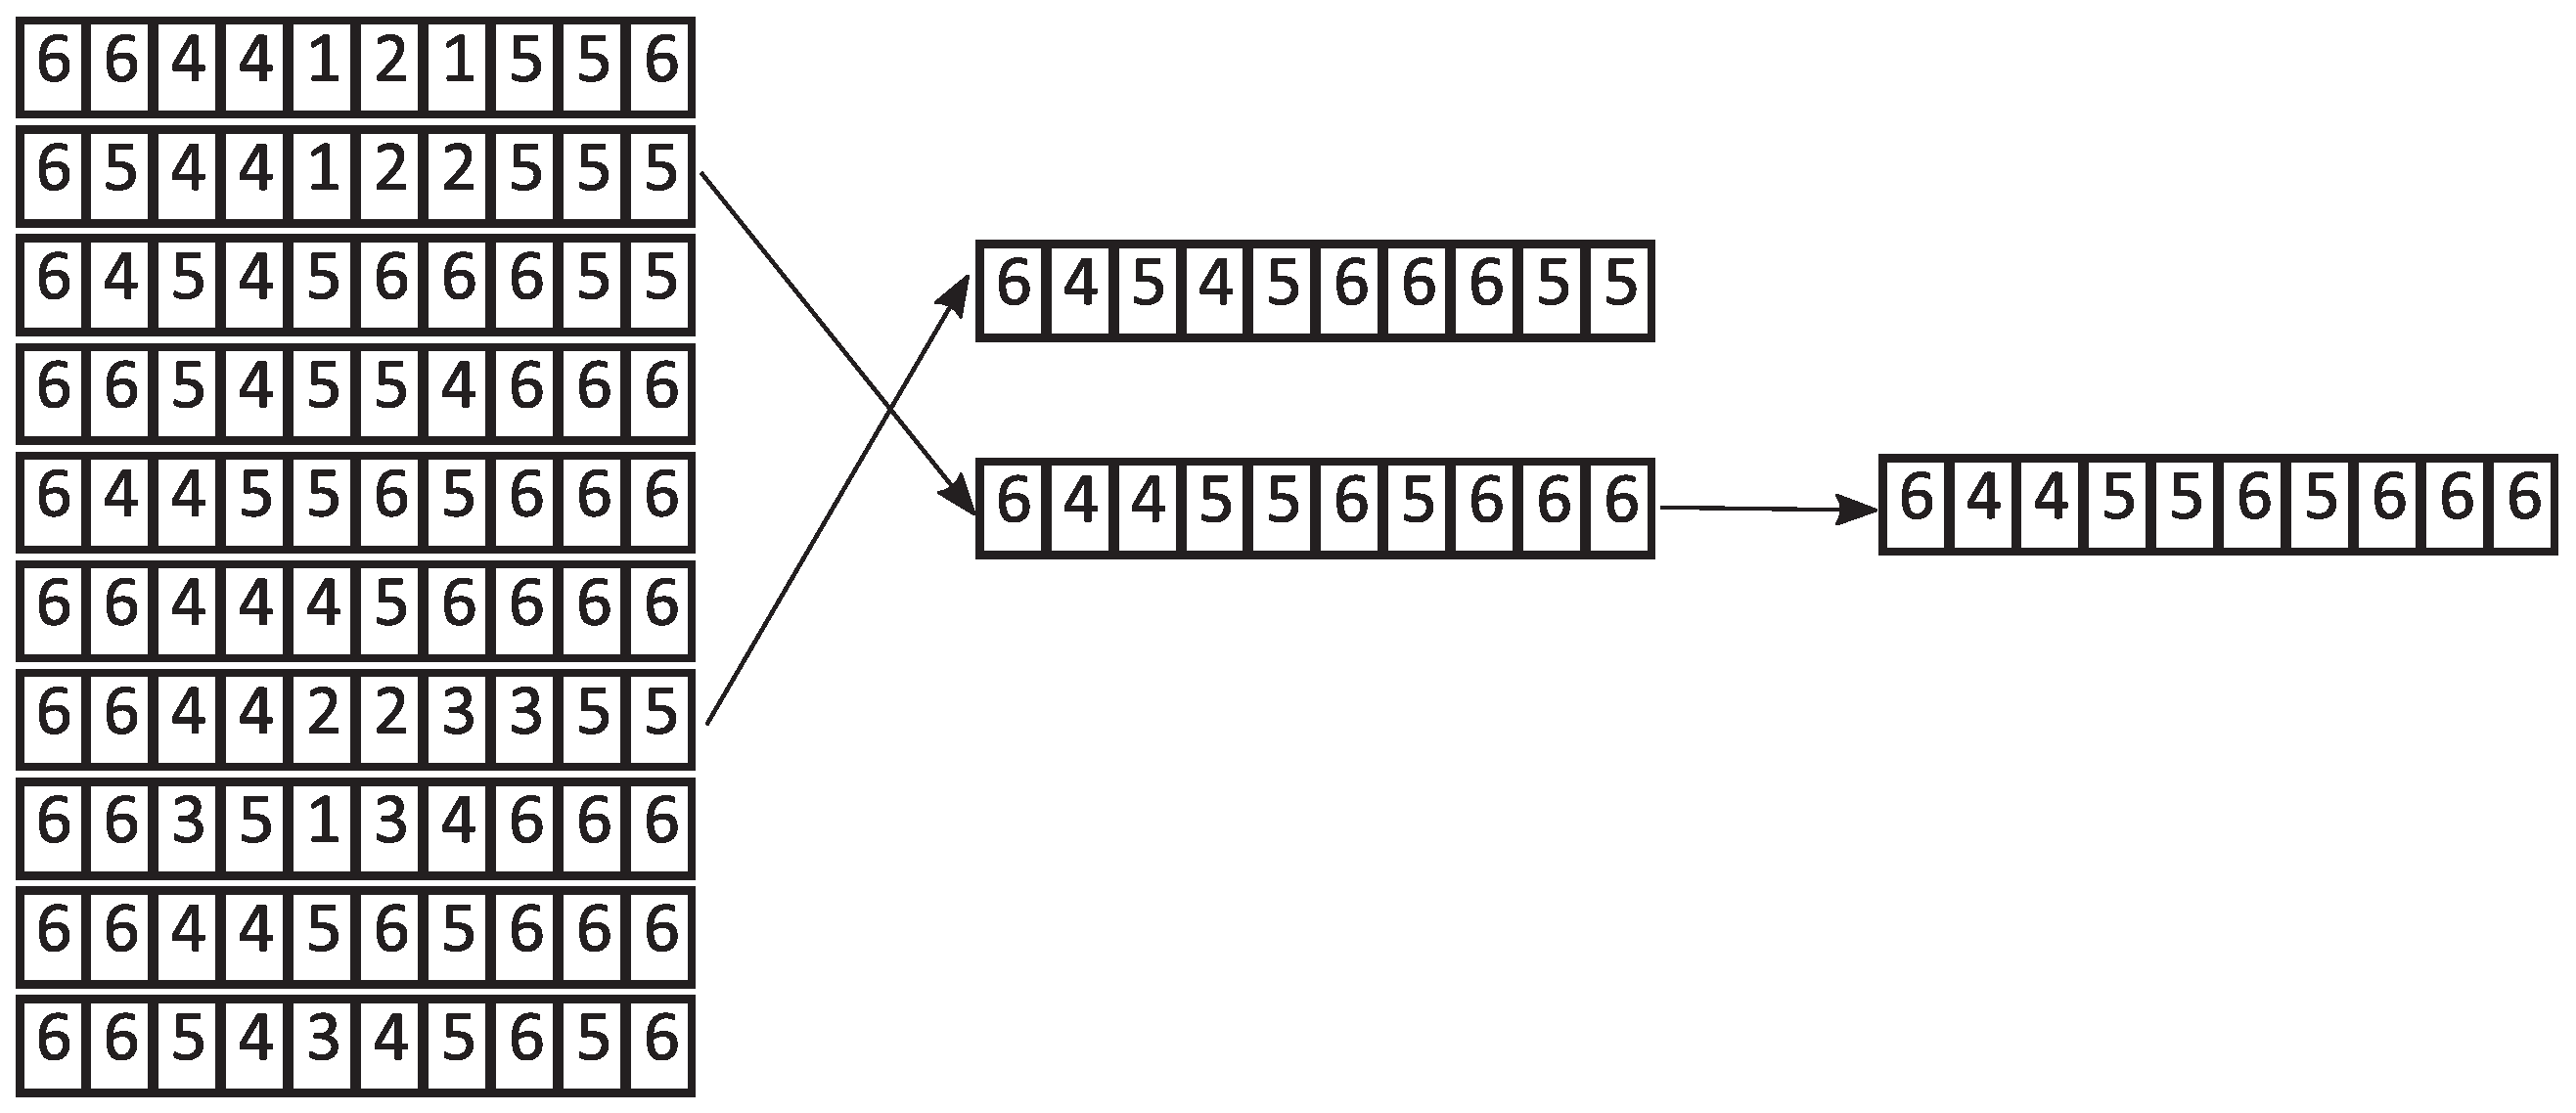
\includegraphics[width=\textwidth]{assets/Anexo/TournamentSelection.eps}
        \end{figure}
    \end{frame}
    \begin{frame}
        \frametitle{Operadores de Selección}
        \textit{Uniform Selection}
        \begin{columns}
            \column{0.5\textwidth}
            $$p_{max} = \frac{\beta}{N_c}$$
            $$p_{min} = \frac{2-\beta}{N_c}$$
            $$1.5 <= \beta <= 2$$             
            $$p_{i} = p_{min} + (p_{max} - p_{min}) \times \frac{N_c - i}{N_c - 1}$$                  
        
            \column{0.5\textwidth}
            \begin{figure}
                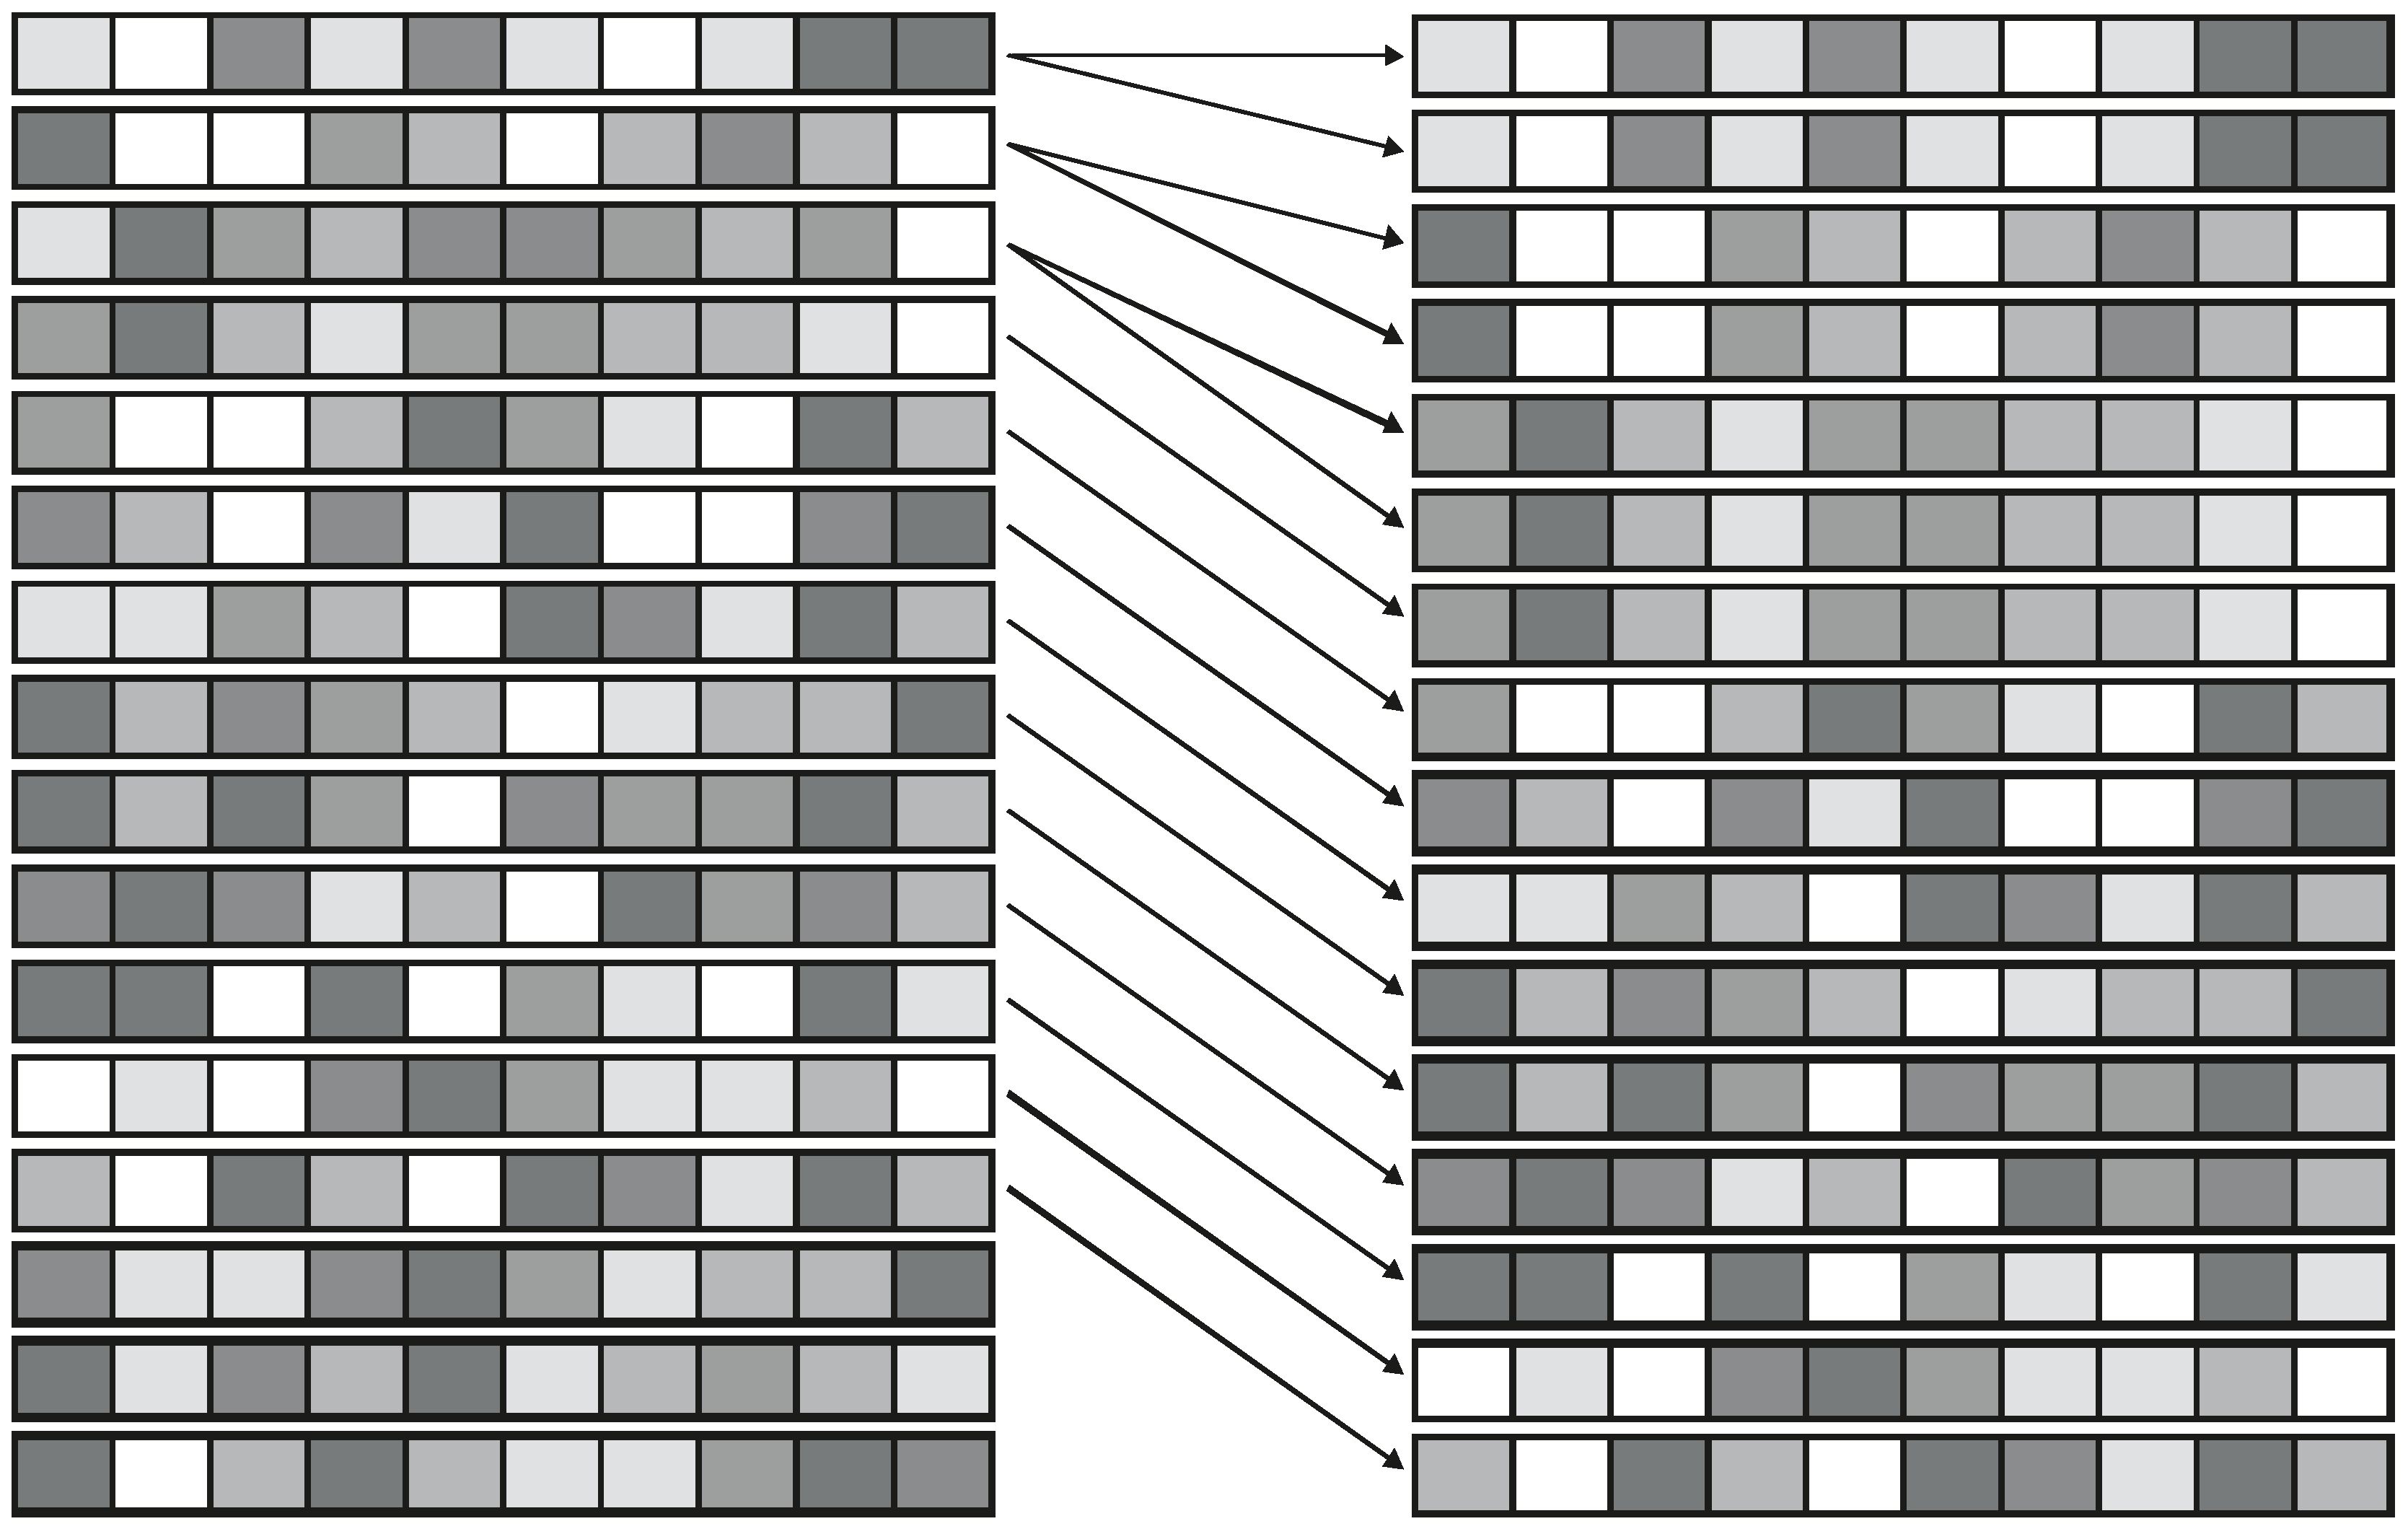
\includegraphics[width=\textwidth]{assets/Anexo/UniformSelection.eps}
            \end{figure}
        \end{columns}

    \end{frame}

    \subsection{Operadores de Cruzamiento}
    \begin{frame}
        \frametitle{Operadores de Selección}
        \textit{SinglePointCrossover}

        \begin{figure}
            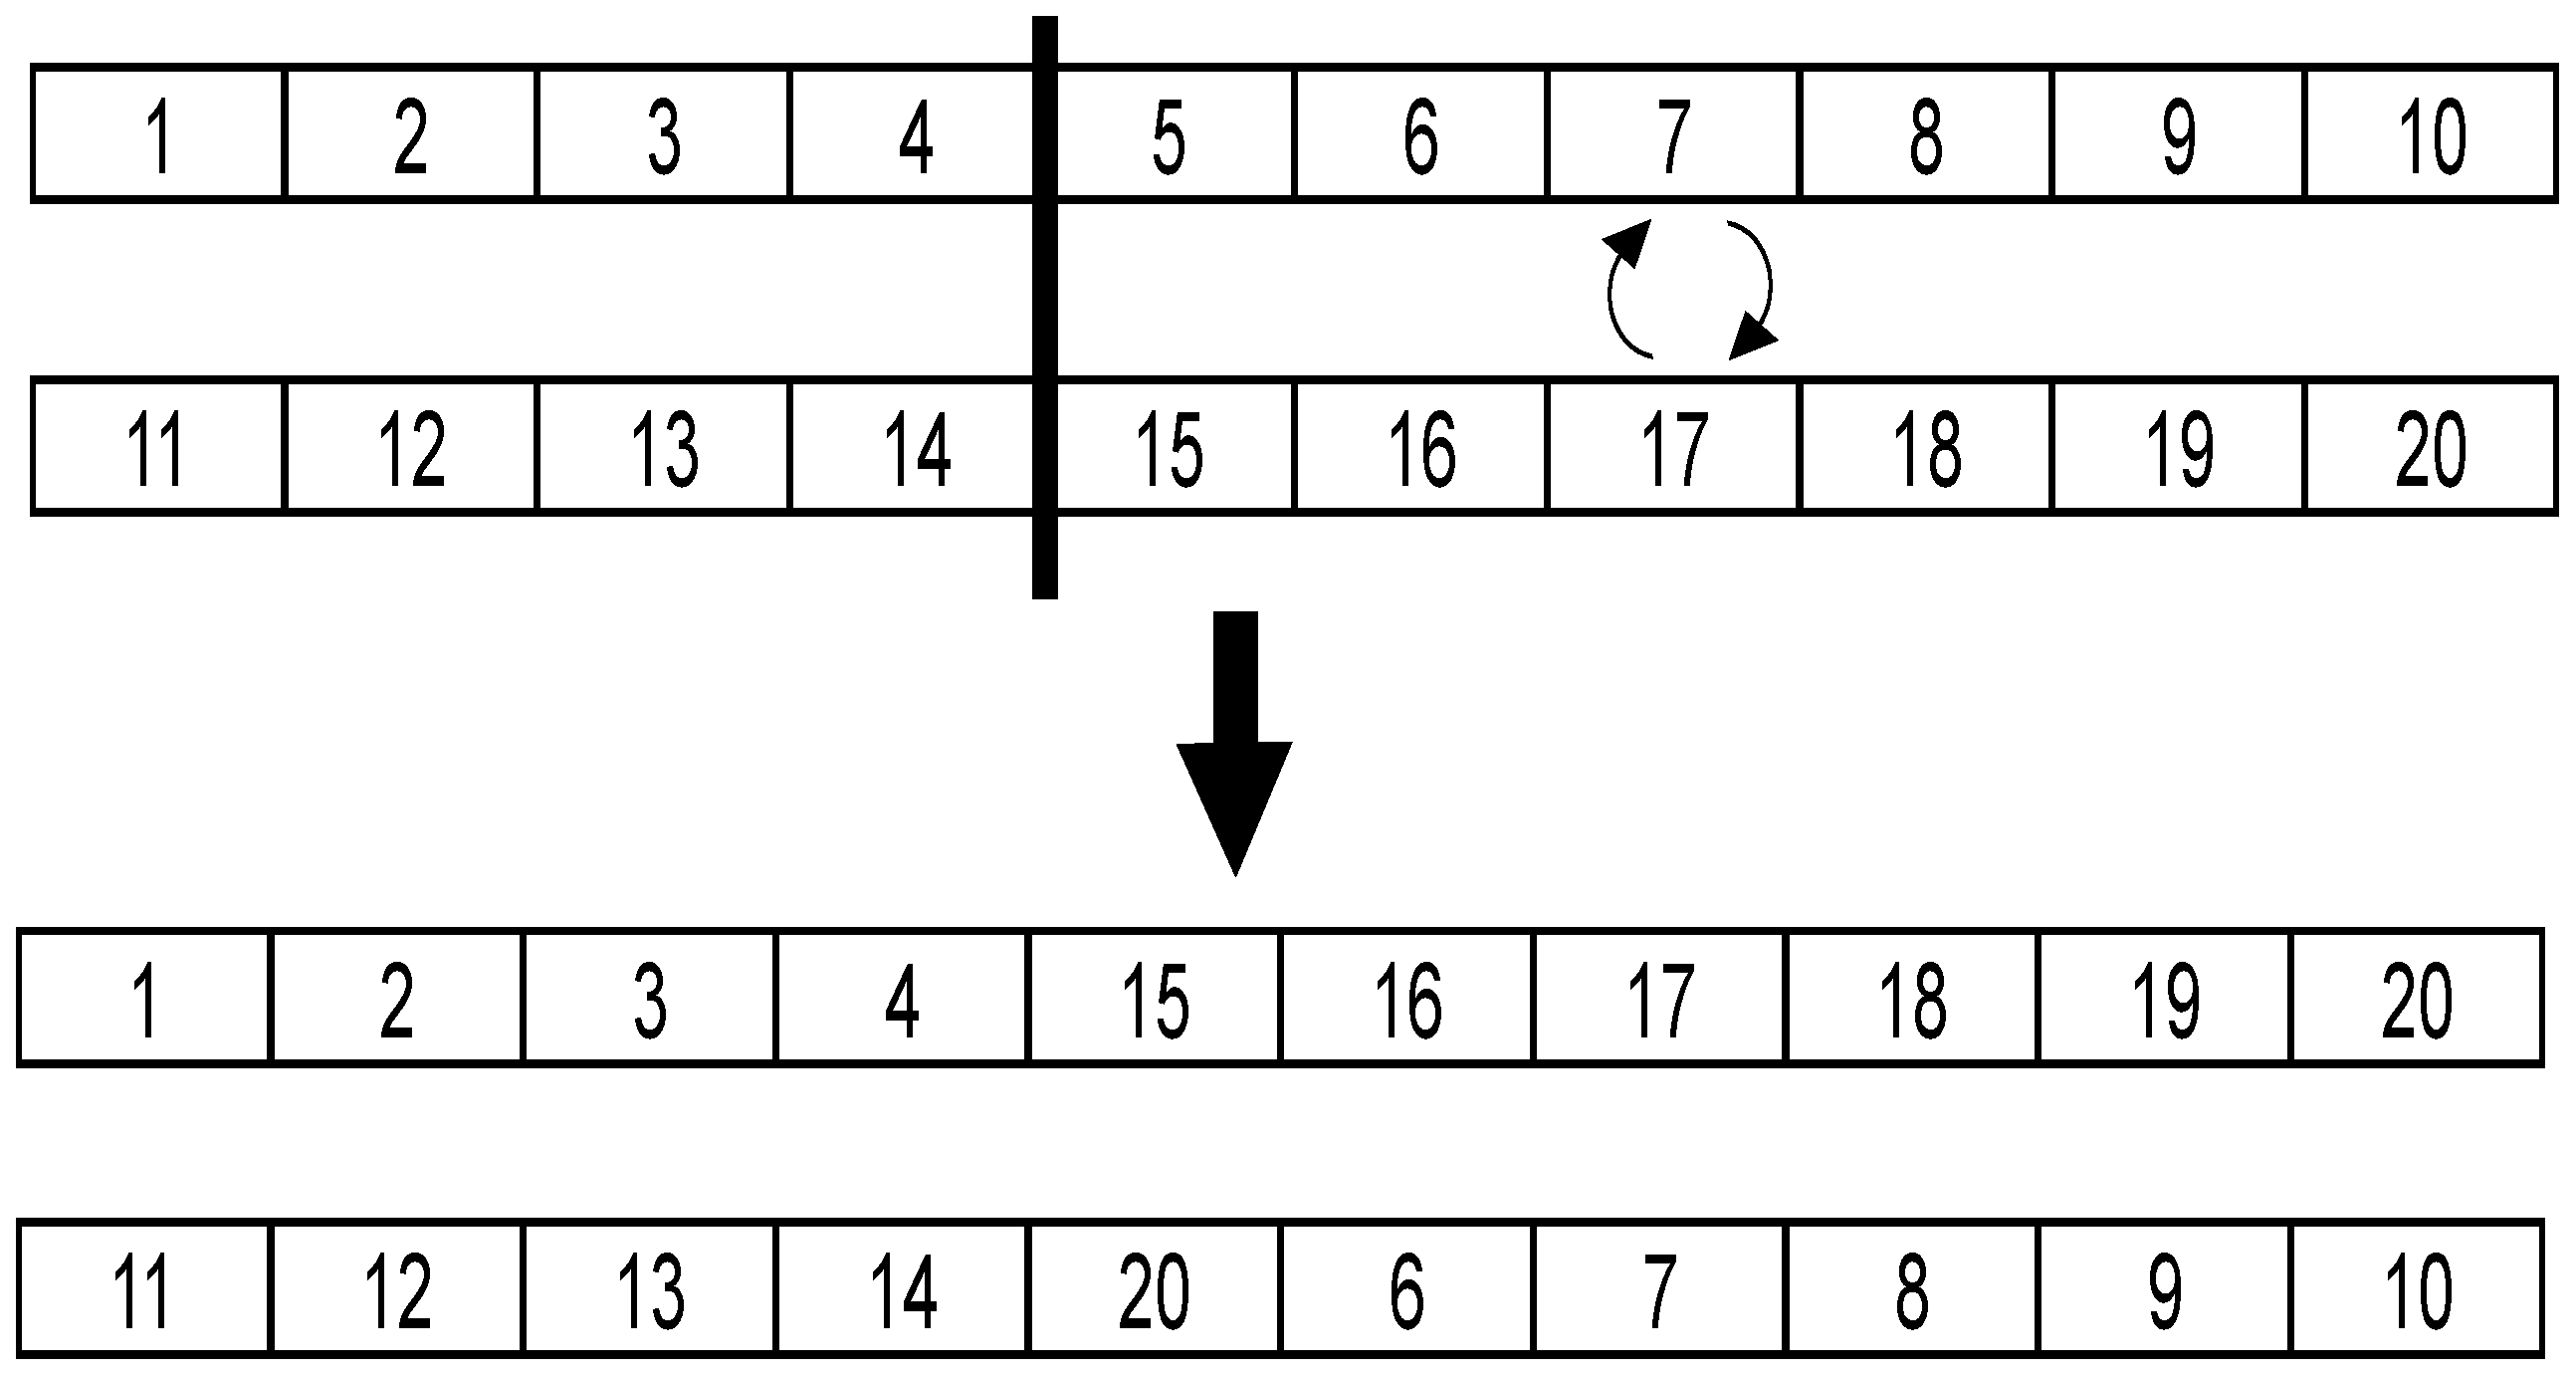
\includegraphics[width=\textwidth]{assets/Anexo/Crossover.eps}
        \end{figure}

    \end{frame}
    \begin{frame}
        \frametitle{Operadores de Selección}
        \textit{SinglePointCrossover}

        \begin{figure}
            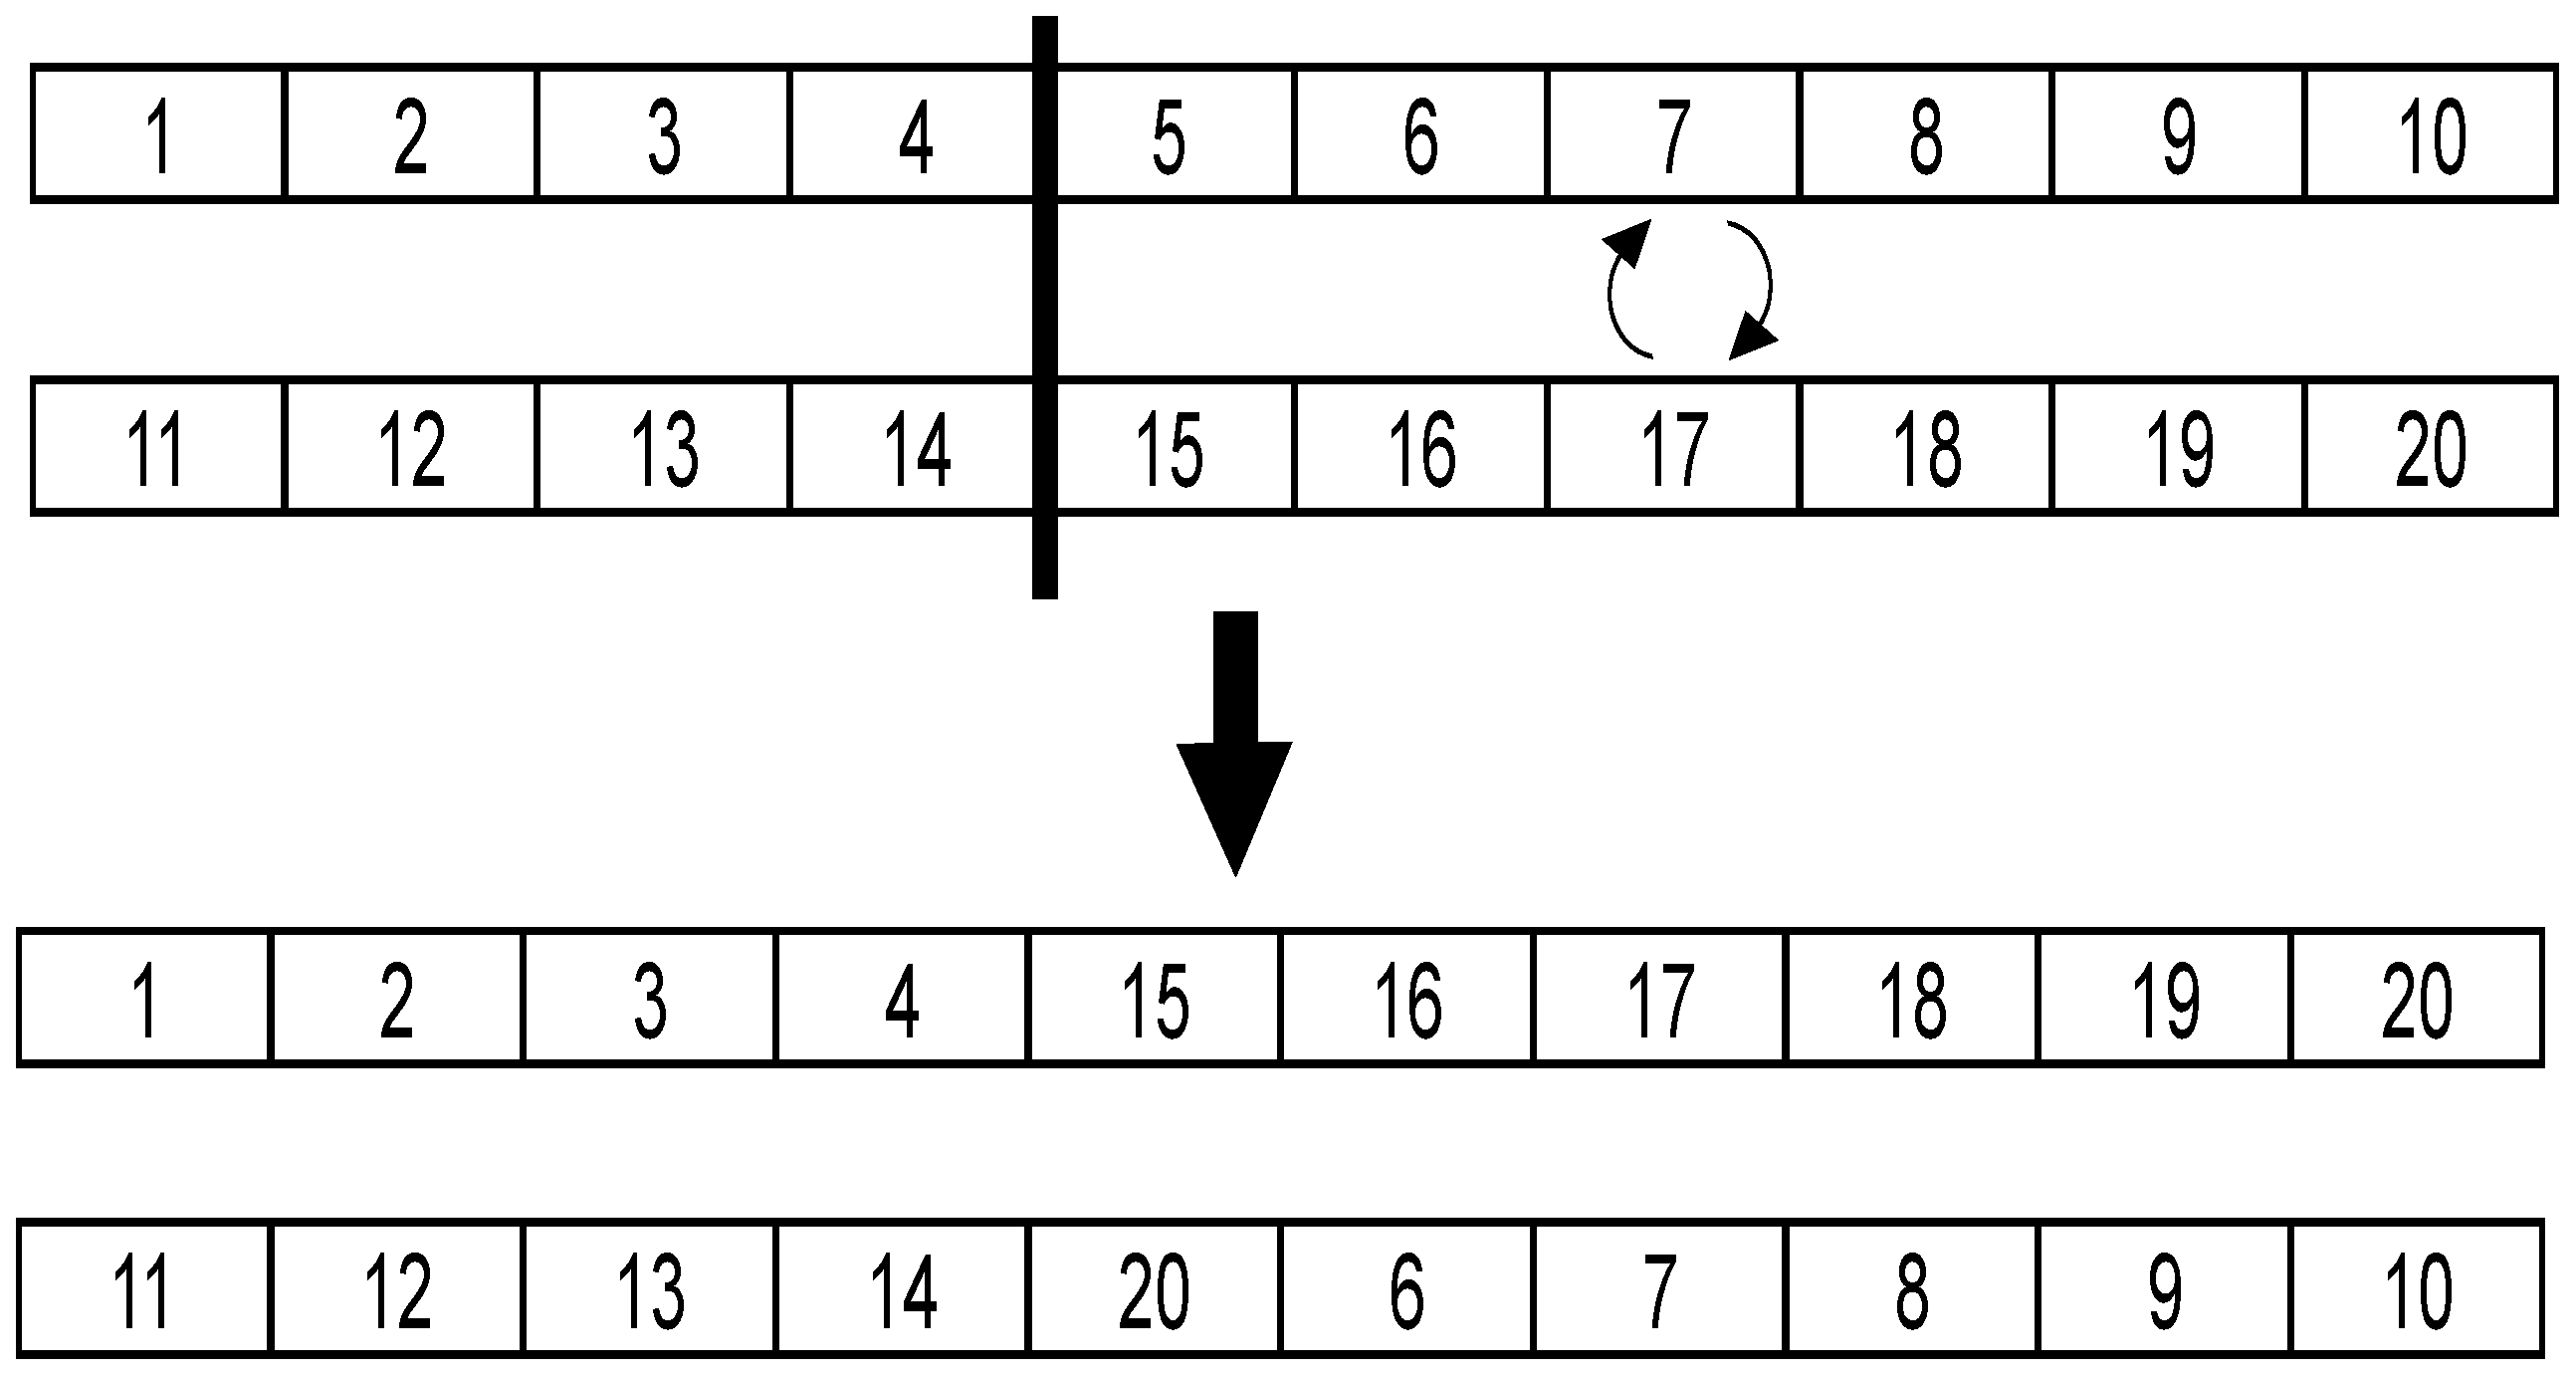
\includegraphics[width=\textwidth]{assets/Anexo/Crossover.eps}
        \end{figure}

    \end{frame}

    \subsection{Operadores de Mutación}
    \begin{frame}
        \frametitle{Operadores de Mutación}
        \textit{SBXCrossover}

        $$
        \begin{cases} 
        \beta_q=\sqrt[d_i+1]{r\alpha} & \text{si $r\leq \frac{1}{\alpha}$} \\ 
        \beta_q=\sqrt[d_i+1]{\frac{1}{2-r\alpha}} &  \text{si $r > \frac{1}{\alpha}$}
        \end{cases}
        $$

        
        \begin{columns}
            \column{0.5\textwidth}
            $$\beta = 1 + 2\frac{y_1-yL}{y_2-y_1}$$
            $$\alpha = 2 - \frac{1}{\beta^{di+1}}$$
    
            $$C_1 = 0.5 ((y_1+y_2)-\beta_q(y_2-y_1))$$
           
            \column{0.5\textwidth}
            $$\beta = 1 + 2 \cdot \frac{yU-y_2}{y_2-y_1}$$
            $$\alpha = 2 - \frac{1}{\beta^{di+1}}$$
    
            $$C_2 = 0.5 ((y_1+y_2)+\beta_q(y_2-y_1))$$
        \end{columns}

    \end{frame}
    \begin{frame}
        \frametitle{Operadores de Mutación}
        \textit{PolynomialMutation}

        $$\Delta_1 = \frac{y-yL}{yU-yL}$$
        $$\Delta_2 = \frac{yU-y}{yU-yL}$$

        $$
        \begin{cases} 
        \Delta_q = \sqrt[di+1]{2r+(1-2r)(1-\Delta_{1})^{di+1}} - 1 & \text{si $r\leq 0.5$} \\ 
        \Delta_q = 1 - \sqrt[di+1]{2(1-r)+2(r-0.5)(1-\Delta_{2})^{di+1}} &  \text{si $r > 0.5$}
        \end{cases}
        $$

        $$y = y + \Delta_q(yU-yL)$$
    \end{frame}


    \subsection{Representación de las soluciones}
    \begin{frame}
        \frametitle{Representación de la solución del problema de diseño}
        Problema de diseño de RDA basado en el costo de tuberías.

        \begin{figure}
            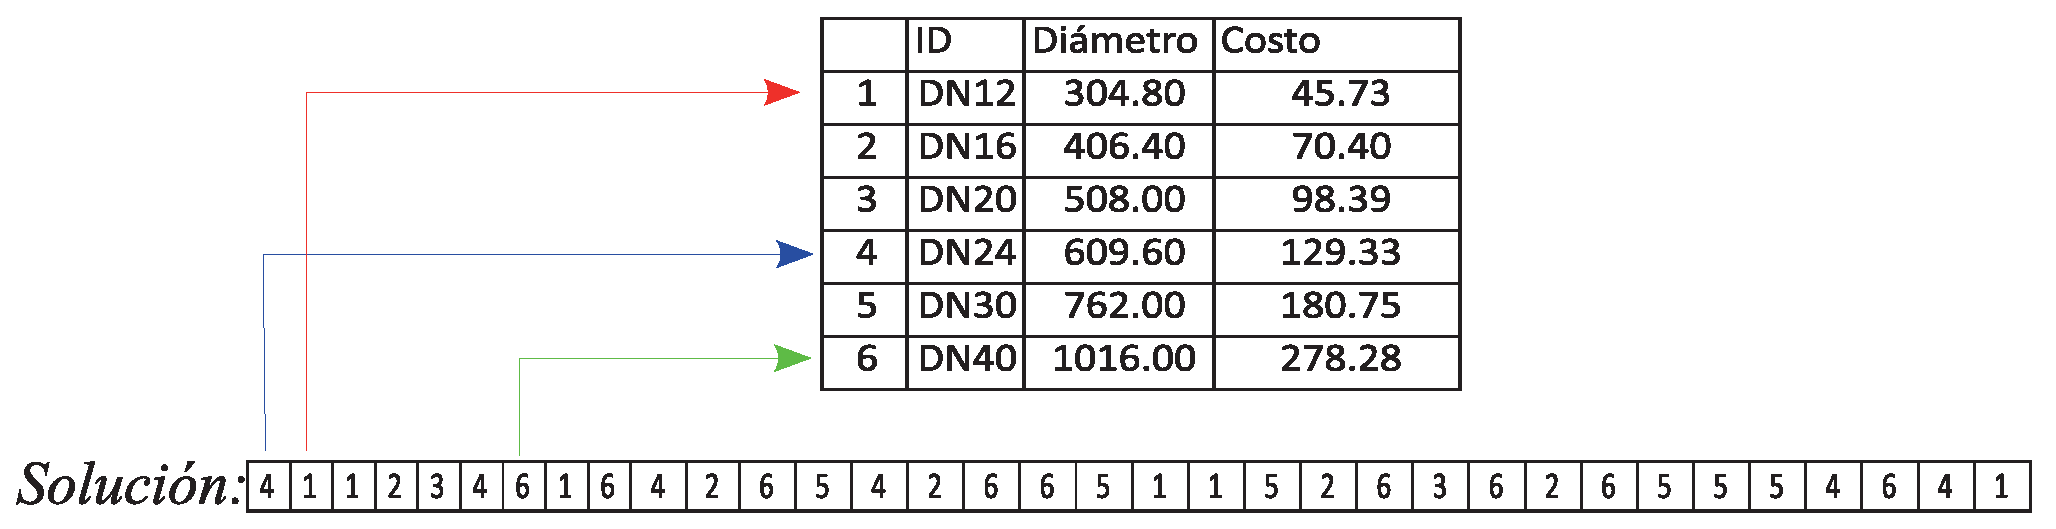
\includegraphics[width=\textwidth]{assets/Anexo/representacion_solucion_monoobjetivo.eps}
        \end{figure}

    \end{frame}

    \begin{frame}
        \frametitle{Representación de la solucion problema operacional}
        Problema de operación basado en el Régimen de bombeo.
        \begin{figure}
            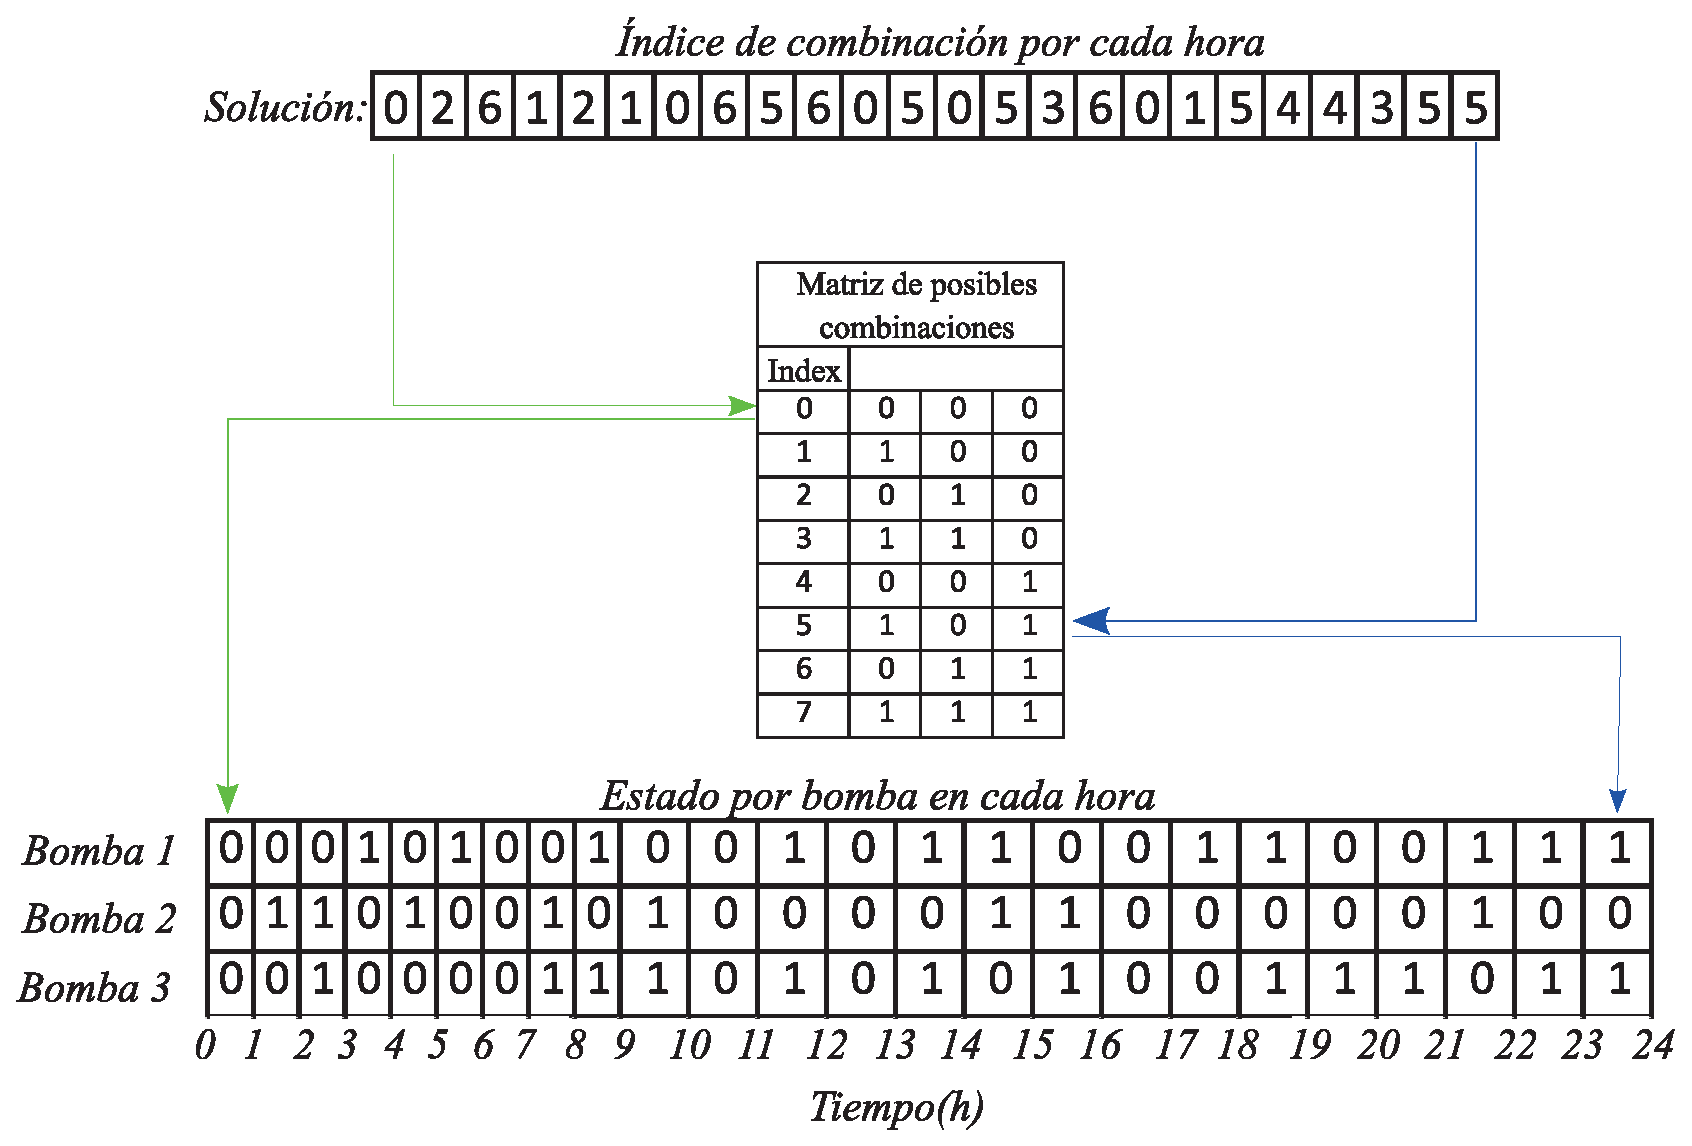
\includegraphics[scale=0.3]{assets/Anexo/representacion_solucion_multiobjetivo.eps}
        \end{figure}

    \end{frame}


\end{document}